\documentclass[UTF8,zihao=-4]{ctexart}

\usepackage[a4paper,margin=2.35cm]{geometry}
\usepackage{amsmath,amssymb}
\usepackage{booktabs}
\usepackage{array}
\usepackage{graphicx}
\usepackage{subcaption}
\usepackage{float}
\usepackage{caption}
\usepackage{xcolor}
\usepackage{hyperref}
\usepackage{enumitem}
\usepackage{multirow}

\hypersetup{
  colorlinks=true,
  linkcolor=blue!55!black,
  urlcolor=blue!55!black,
  citecolor=blue!55!black
}

\captionsetup{font=small,labelfont=bf}
\setlist[itemize]{leftmargin=2em,itemsep=0.2em}
\setlist[enumerate]{leftmargin=2em,itemsep=0.2em}
\renewcommand{\arraystretch}{1.18}
\graphicspath{{results/figures/}}

\title{\bfseries Mesa ABM 双边平台竞争实验报告}
\author{Agent-Based Modeling with Mesa}
\date{\today}

\begin{document}
\maketitle

\begin{abstract}
本文基于 Mesa 多智能体仿真框架，研究双边平台竞争中个体异质性、补贴投放、冷启动资源结构与商户多归属机制对市场锁定和平台共存的影响。模型将用户与商户分别表示为具有差异化偏好、惯性、补贴敏感度和随机扰动的智能体，并通过双边网络效应连接用户侧需求和商户侧供给。实验结果表明：平台竞争存在明显的临界区间；双边精准补贴相较统一补贴和随机补贴能够显著降低跨越临界规模所需预算；冷启动成功不仅取决于种子规模，还取决于用户侧与商户侧资源是否同步达到启动阈值；低成本多归属有助于平台共存。进一步的机制消融显示，双边网络效应和多归属机制是弱势平台跨越临界区的关键来源；ABM 与 ODE 对比表明，ABM 在保持平均场趋势的同时，能够揭示临界区内由个体异质性和随机路径导致的结果分布。
\end{abstract}

\section{实验背景与研究问题}

双边平台同时连接用户侧和商户侧。用户选择平台时受到平台服务质量、价格补贴和商户供给规模影响；商户选择平台时则受到用户流量、平台抽成、补贴和多归属成本影响。因此，双边平台竞争具有典型的交叉网络效应：用户越多，越能吸引商户；商户供给越充分，又会进一步吸引用户。

在强网络效应环境下，市场可能出现三类宏观结果：平台 A 锁定、平台 B 锁定和双平台共存。传统均值模型通常关注总体份额演化，难以解释个体差异、定向补贴、多归属行为和随机路径依赖如何共同塑造最终格局。ABM 的价值在于从微观主体决策出发，观察大量异质个体的局部选择如何累积为宏观市场结构。

在本文的整体建模框架中，ODE 与 ABM 的作用并不相同。宏观 ODE 模型刻画的是平均场意义下的双边网络效应和市场份额演化，适合判断平台竞争是否存在锁定、共存和临界区间；ABM 则进一步把平均主体拆解为具有偏好差异、惯性、补贴敏感度和多归属行为的微观主体，用于回答这些宏观现象在个体层面通过何种机制形成。因此，ABM 不是对 ODE 的简单替代，而是对 ODE 的微观扩展：它既检验平均场结论在随机个体环境下是否仍然成立，也揭示 ODE 无法直接表达的结果分布和路径依赖。

本文围绕四个关键问题设计实验：

\begin{enumerate}
  \item 个体异质性是否削弱赢家通吃，还是会放大初始优势？
  \item 在等预算约束下，精准补贴是否优于统一补贴和随机补贴？
  \item 冷启动阶段用户侧和商户侧资源如何共同决定启动边界？
  \item 商户多归属成本和有效供给贡献如何影响平台共存？
\end{enumerate}

为增强参数解释性，本文将主要变量与现实策略含义对应如下：$u_A(0)$ 表示平台 A 的初始用户基础或活跃用户占比；$m_A(0)$ 表示初始商户覆盖和供给密度；$B$ 表示补贴预算；$k_M$ 表示商户跨平台经营成本、排他协议成本或规则复杂度；$\rho$ 表示多归属商户在单个平台上的有效曝光和供给贡献；$\sigma_\theta$ 表示用户与商户偏好差异程度。后续实验不追求对某一真实平台的精确预测，而是在合理参数范围内识别机制方向、临界条件和策略稳健性。

\section{模型设定}

\subsection{主体与平台选择}

模型包含两类智能体：用户 agent 和商户 agent。用户在平台 A 与平台 B 之间选择；商户可以选择 A-only、B-only 或 multi-home。每个主体具有个体属性，包括价格敏感度、补贴敏感度、质量偏好、惯性、流量敏感度、抽成敏感度和随机偏好扰动。异质性参数控制这些属性在主体之间的离散程度。

记平台 A 的用户份额为 $u_A(t)$，平台 A 的有效商户供给份额为 $m_A^{eff}(t)$，则综合市场份额定义为
\begin{equation}
L_A(t)=\frac{u_A(t)+m_A^{eff}(t)}{2}.
\end{equation}
本文将 $L_A$ 作为衡量平台 A 市场地位的核心指标。

\subsection{商户多归属}

商户处于三种状态：
\begin{equation}
A\text{-only},\quad B\text{-only},\quad multi\text{-home}.
\end{equation}
若商户多归属，则其对两个平台均产生有效供给贡献。记多归属有效供给贡献为 $\rho$，则
\begin{equation}
M_A^{eff}=M_{A-only}+\rho M_{multi}, \qquad
M_B^{eff}=M_{B-only}+\rho M_{multi}.
\end{equation}
多归属成本越高，商户越倾向于选择单一平台；$\rho$ 越高，多归属商户对单个平台的可见供给贡献越强。

\subsection{结果判定与重复实验}

仿真结束时，根据最终综合份额 $L_A(T)$ 判定市场状态：
\begin{equation}
\begin{cases}
L_A(T)\ge 0.8, & \text{平台 A 锁定},\\
L_A(T)\le 0.2, & \text{平台 B 锁定},\\
0.2<L_A(T)<0.8, & \text{双平台共存}.
\end{cases}
\end{equation}
平台 A 的成功概率定义为
\begin{equation}
P(L_A(T)>0.6).
\end{equation}
主要实验采用多随机种子重复运行，细粒度临界区间实验每个参数点重复 50 次，以降低概率估计误差。

\section{实验 A：临界区个体异质性}

\subsection{实验目的与设计}

本实验研究个体异质性是否会改变市场锁定概率和最终份额分布。平台 A 初始仅具有轻微优势：
\[
u_A(0)=0.52,\qquad m_A(0)=0.52,
\]
双边网络效应参数设为 $\alpha=\beta=2.3$。异质性强度取
\[
\sigma_\theta\in\{0,0.25,0.50,0.75,1.00,1.25,1.50,2.00\},
\]
每组重复运行 30 次。

\begin{figure}[H]
  \centering
  \begin{subfigure}{0.49\textwidth}
    \centering
    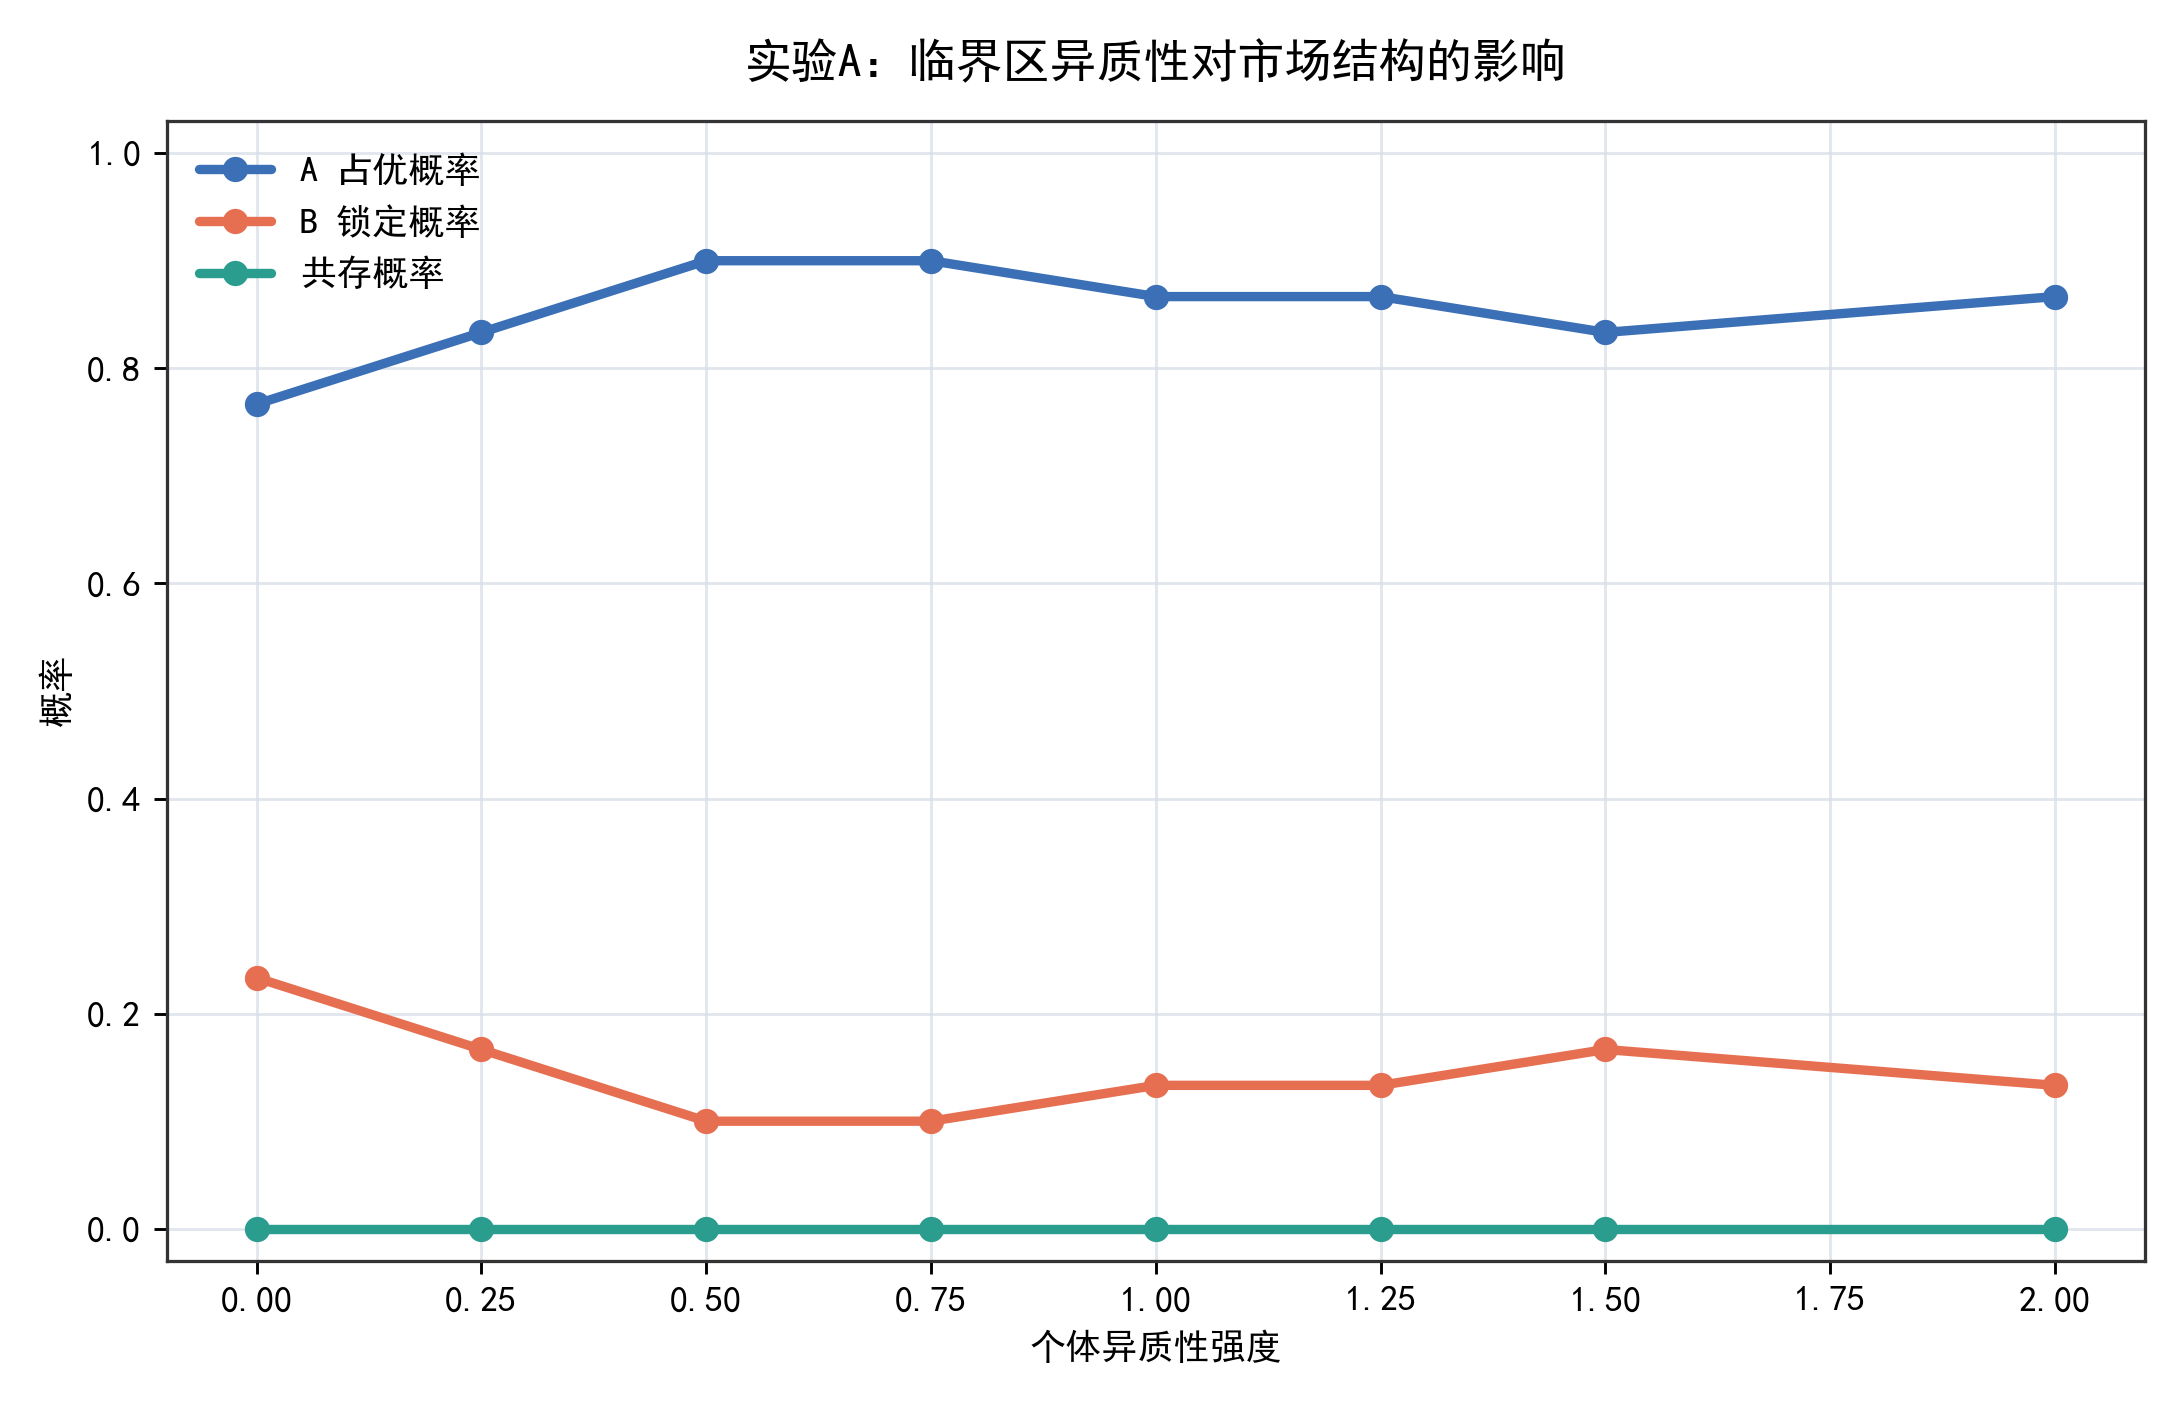
\includegraphics[width=\textwidth]{revised_A_heterogeneity_probabilities.png}
    \caption{异质性对市场结构概率的影响}
  \end{subfigure}
  \hfill
  \begin{subfigure}{0.49\textwidth}
    \centering
    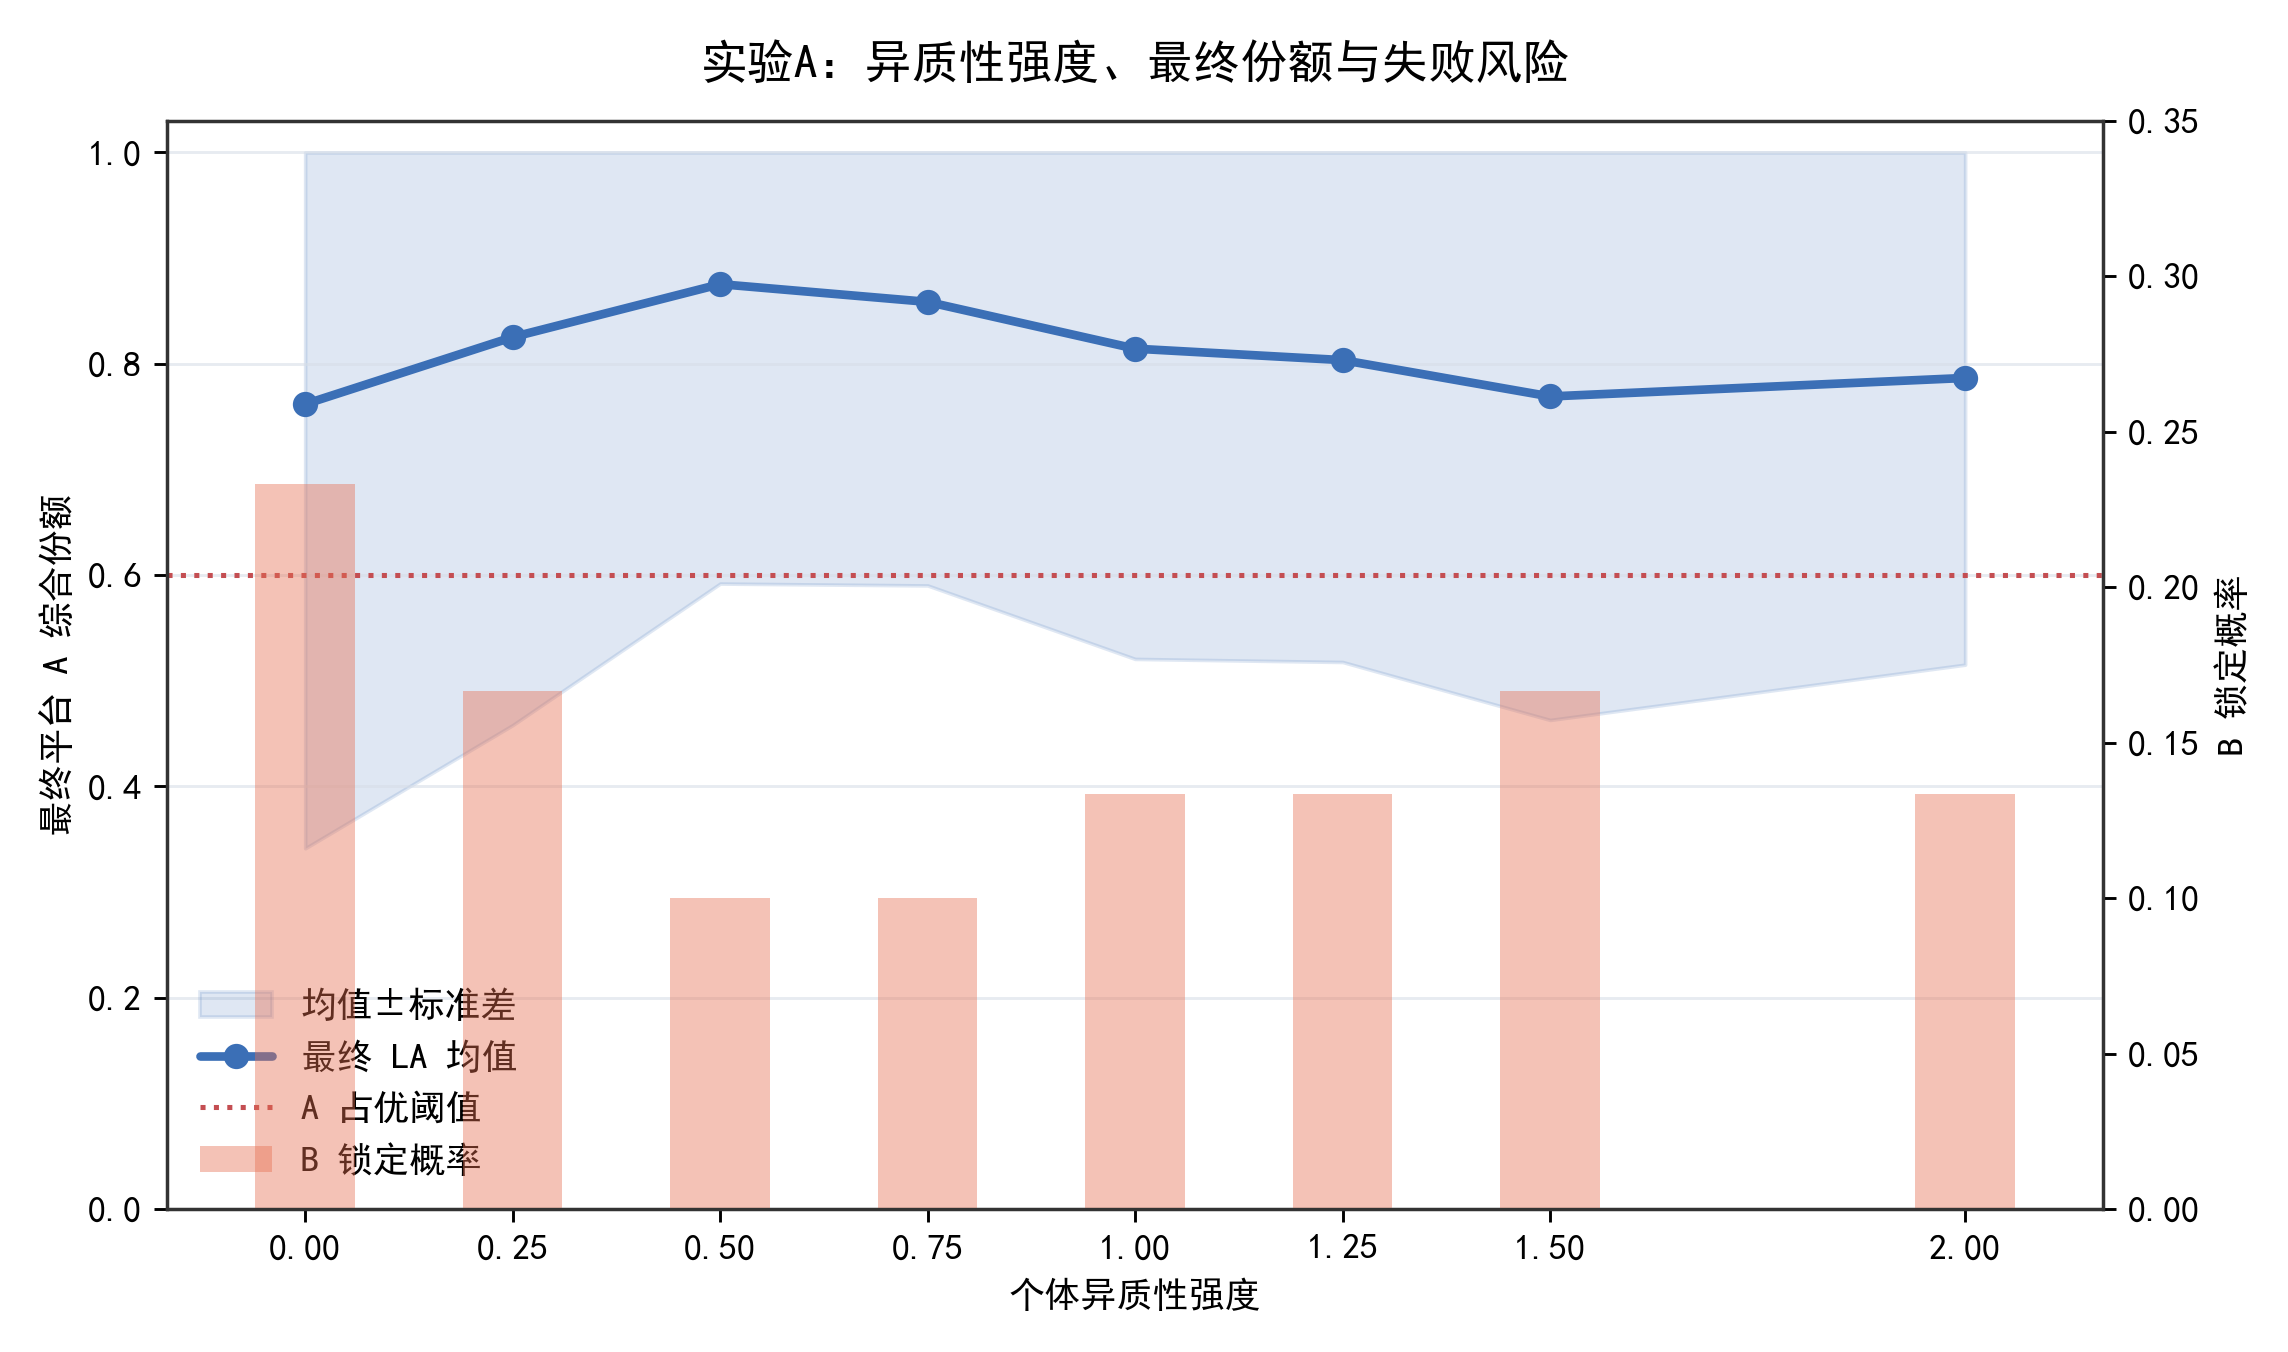
\includegraphics[width=\textwidth]{revised_A_heterogeneity_boxplot.png}
    \caption{最终 $L_A$ 分布}
  \end{subfigure}
  \caption{临界区个体异质性实验结果}
  \label{fig:exp-a}
\end{figure}

\begin{table}[H]
\centering
\caption{异质性强度与市场结果}
\label{tab:exp-a}
\begin{tabular}{rrrrrr}
\toprule
$\sigma_\theta$ & $\bar L_A$ & $sd(L_A)$ & A 成功概率 & A 锁定概率 & 集中度 \\
\midrule
0.00 & 0.762 & 0.420 & 0.767 & 0.767 & 0.979 \\
0.25 & 0.825 & 0.367 & 0.833 & 0.833 & 0.972 \\
0.50 & 0.875 & 0.283 & 0.900 & 0.900 & 0.937 \\
0.75 & 0.859 & 0.268 & 0.900 & 0.900 & 0.896 \\
1.00 & 0.814 & 0.294 & 0.867 & 0.867 & 0.864 \\
1.25 & 0.803 & 0.286 & 0.867 & 0.867 & 0.842 \\
1.50 & 0.769 & 0.306 & 0.833 & 0.833 & 0.826 \\
2.00 & 0.787 & 0.271 & 0.867 & 0.867 & 0.807 \\
\bottomrule
\end{tabular}
\end{table}

结果显示，个体异质性的作用并非单调。无异质性时，平台 A 锁定概率为 0.767，说明即使 A 具有轻微初始优势，随机路径仍可能导致 B 锁定。当异质性提升至 0.50--0.75 时，A 成功概率上升到 0.900，说明中等异质性可能使部分高敏感主体更快响应 A 的初始优势，从而放大双边正反馈。继续提高异质性后，市场集中度由 0.937 降至 0.807，表明强异质性会削弱赢家通吃强度，使最终份额更加分散。

\begin{figure}[H]
  \centering
  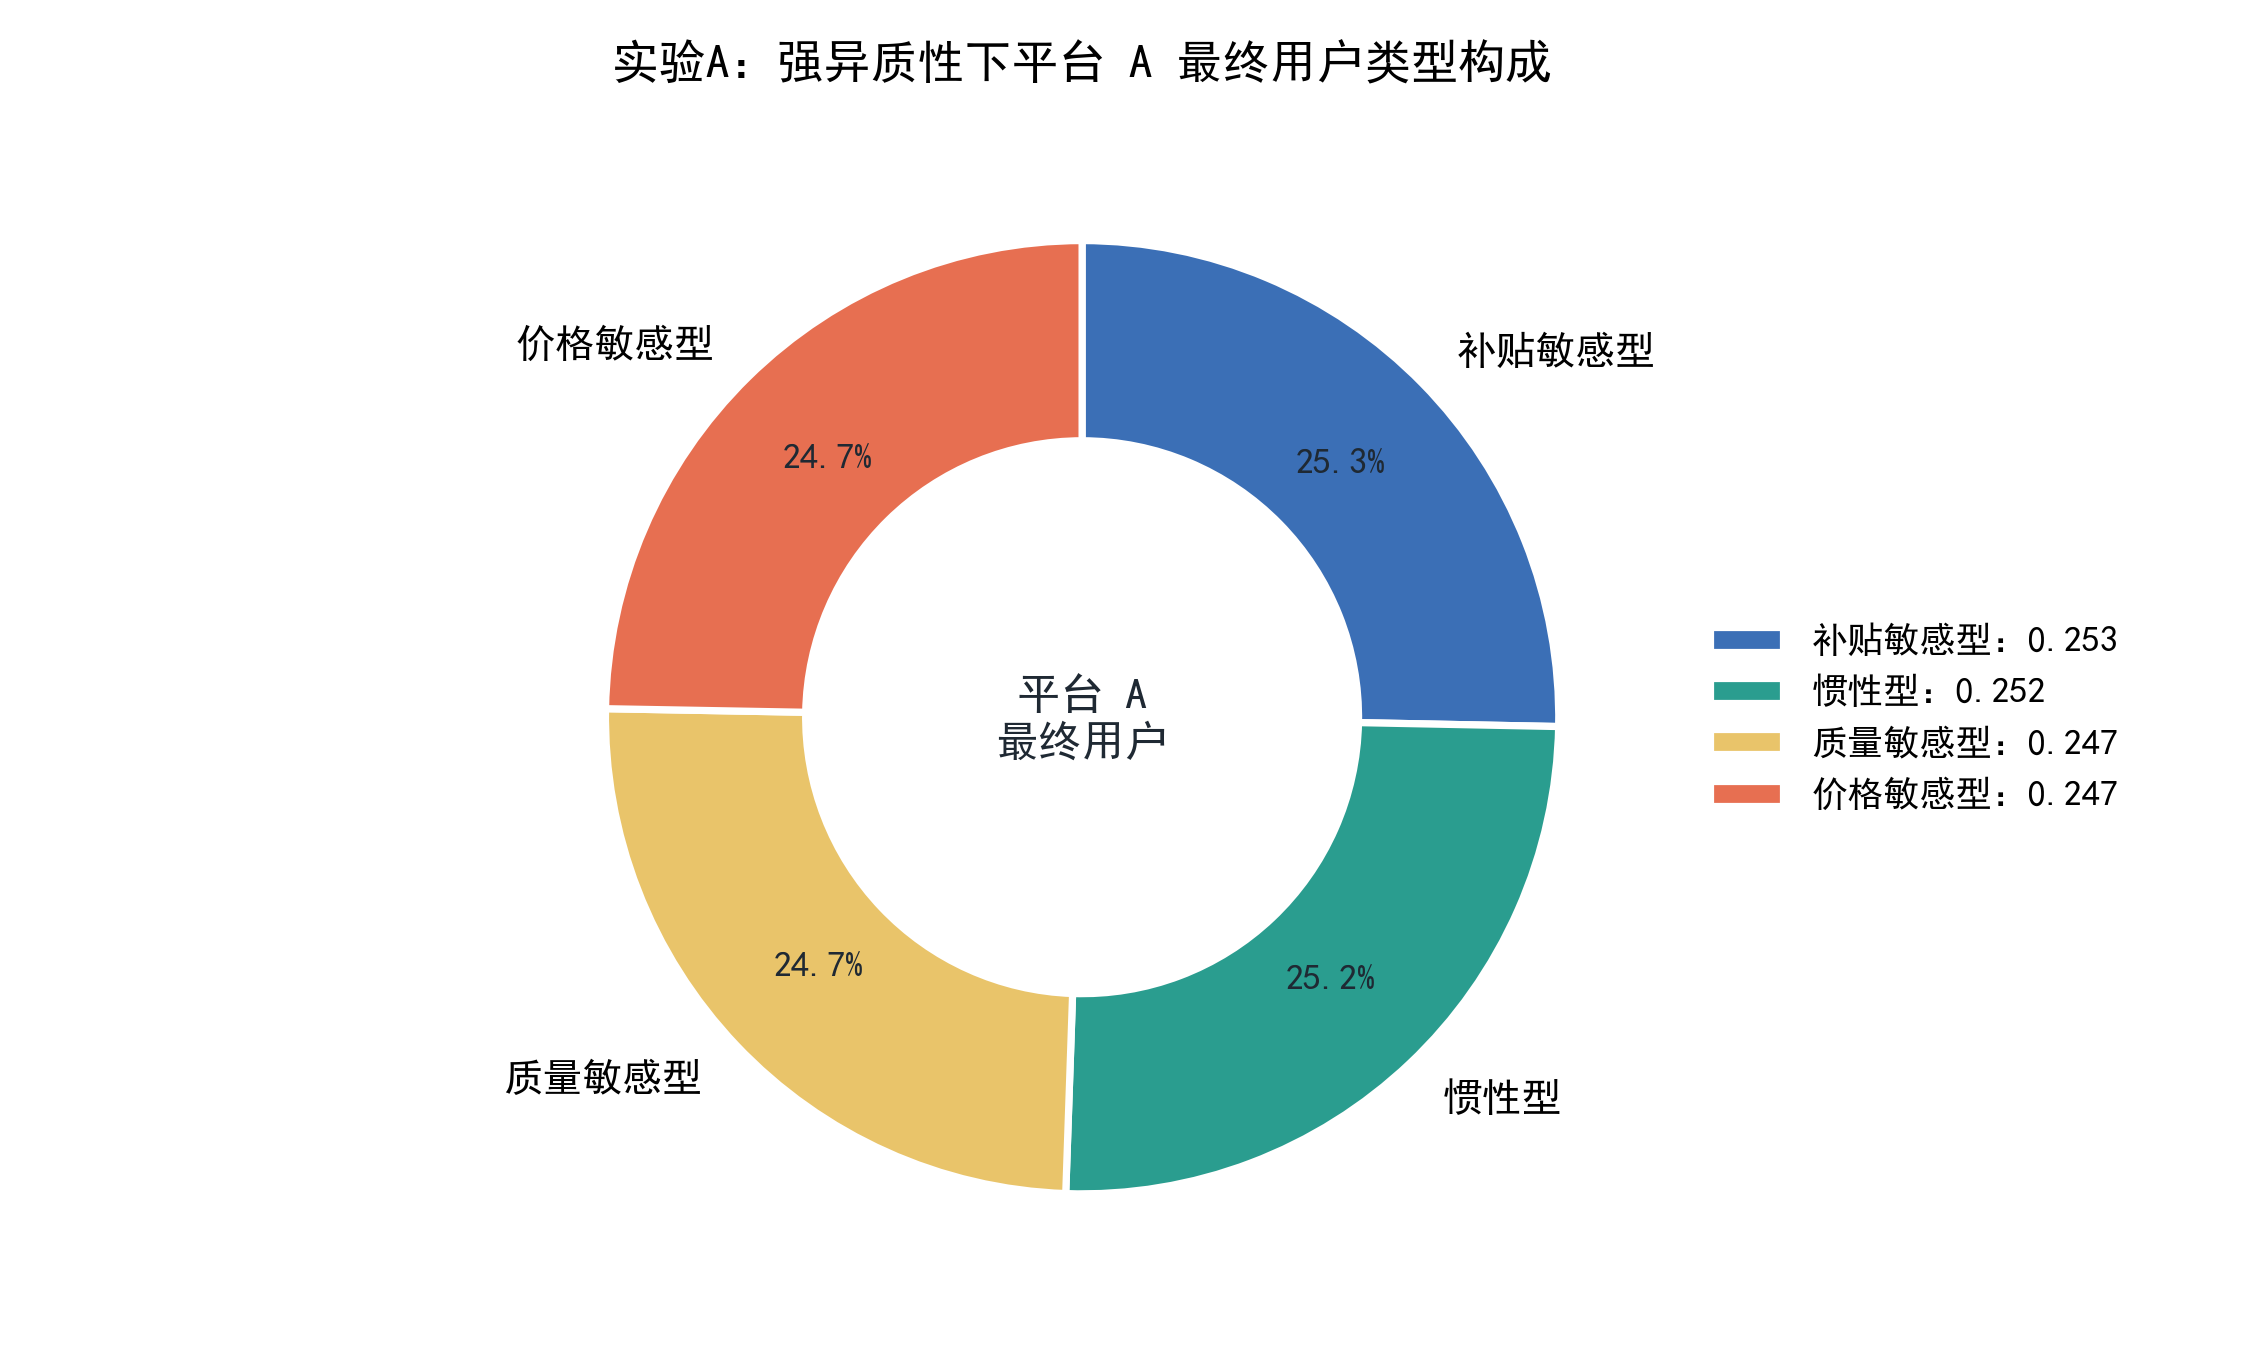
\includegraphics[width=0.72\textwidth]{revised_A_user_segment_distribution.png}
  \caption{强异质性条件下不同用户类型的平台 A 留存比例}
  \label{fig:user-segment}
\end{figure}

图 \ref{fig:user-segment} 进一步解释了异质性机制：不同用户类型最终均更多留在平台 A，但类型之间存在差异。结合商户类型分布可以发现，流量敏感型商户更容易被优势平台吸引，这说明用户侧优势通过商户侧流量收益被进一步放大。

\section{实验 B：等预算补贴策略}

\subsection{实验目的与设计}

本实验研究在相同补贴预算下，不同补贴策略帮助弱势平台跨越临界规模的能力。平台 A 初始处于劣势：
\[
u_A(0)=0.30,\qquad m_A(0)=0.30,
\]
网络效应参数设为 $\alpha=\beta=2.5$，异质性强度设为 $\sigma_\theta=0.8$。比较统一补贴、随机补贴和双边精准补贴等策略。细粒度扫描在预算区间 $B\in[120,300]$ 内进行，每个预算--策略组合重复 50 次。

\begin{figure}[H]
  \centering
  \begin{subfigure}{0.49\textwidth}
    \centering
    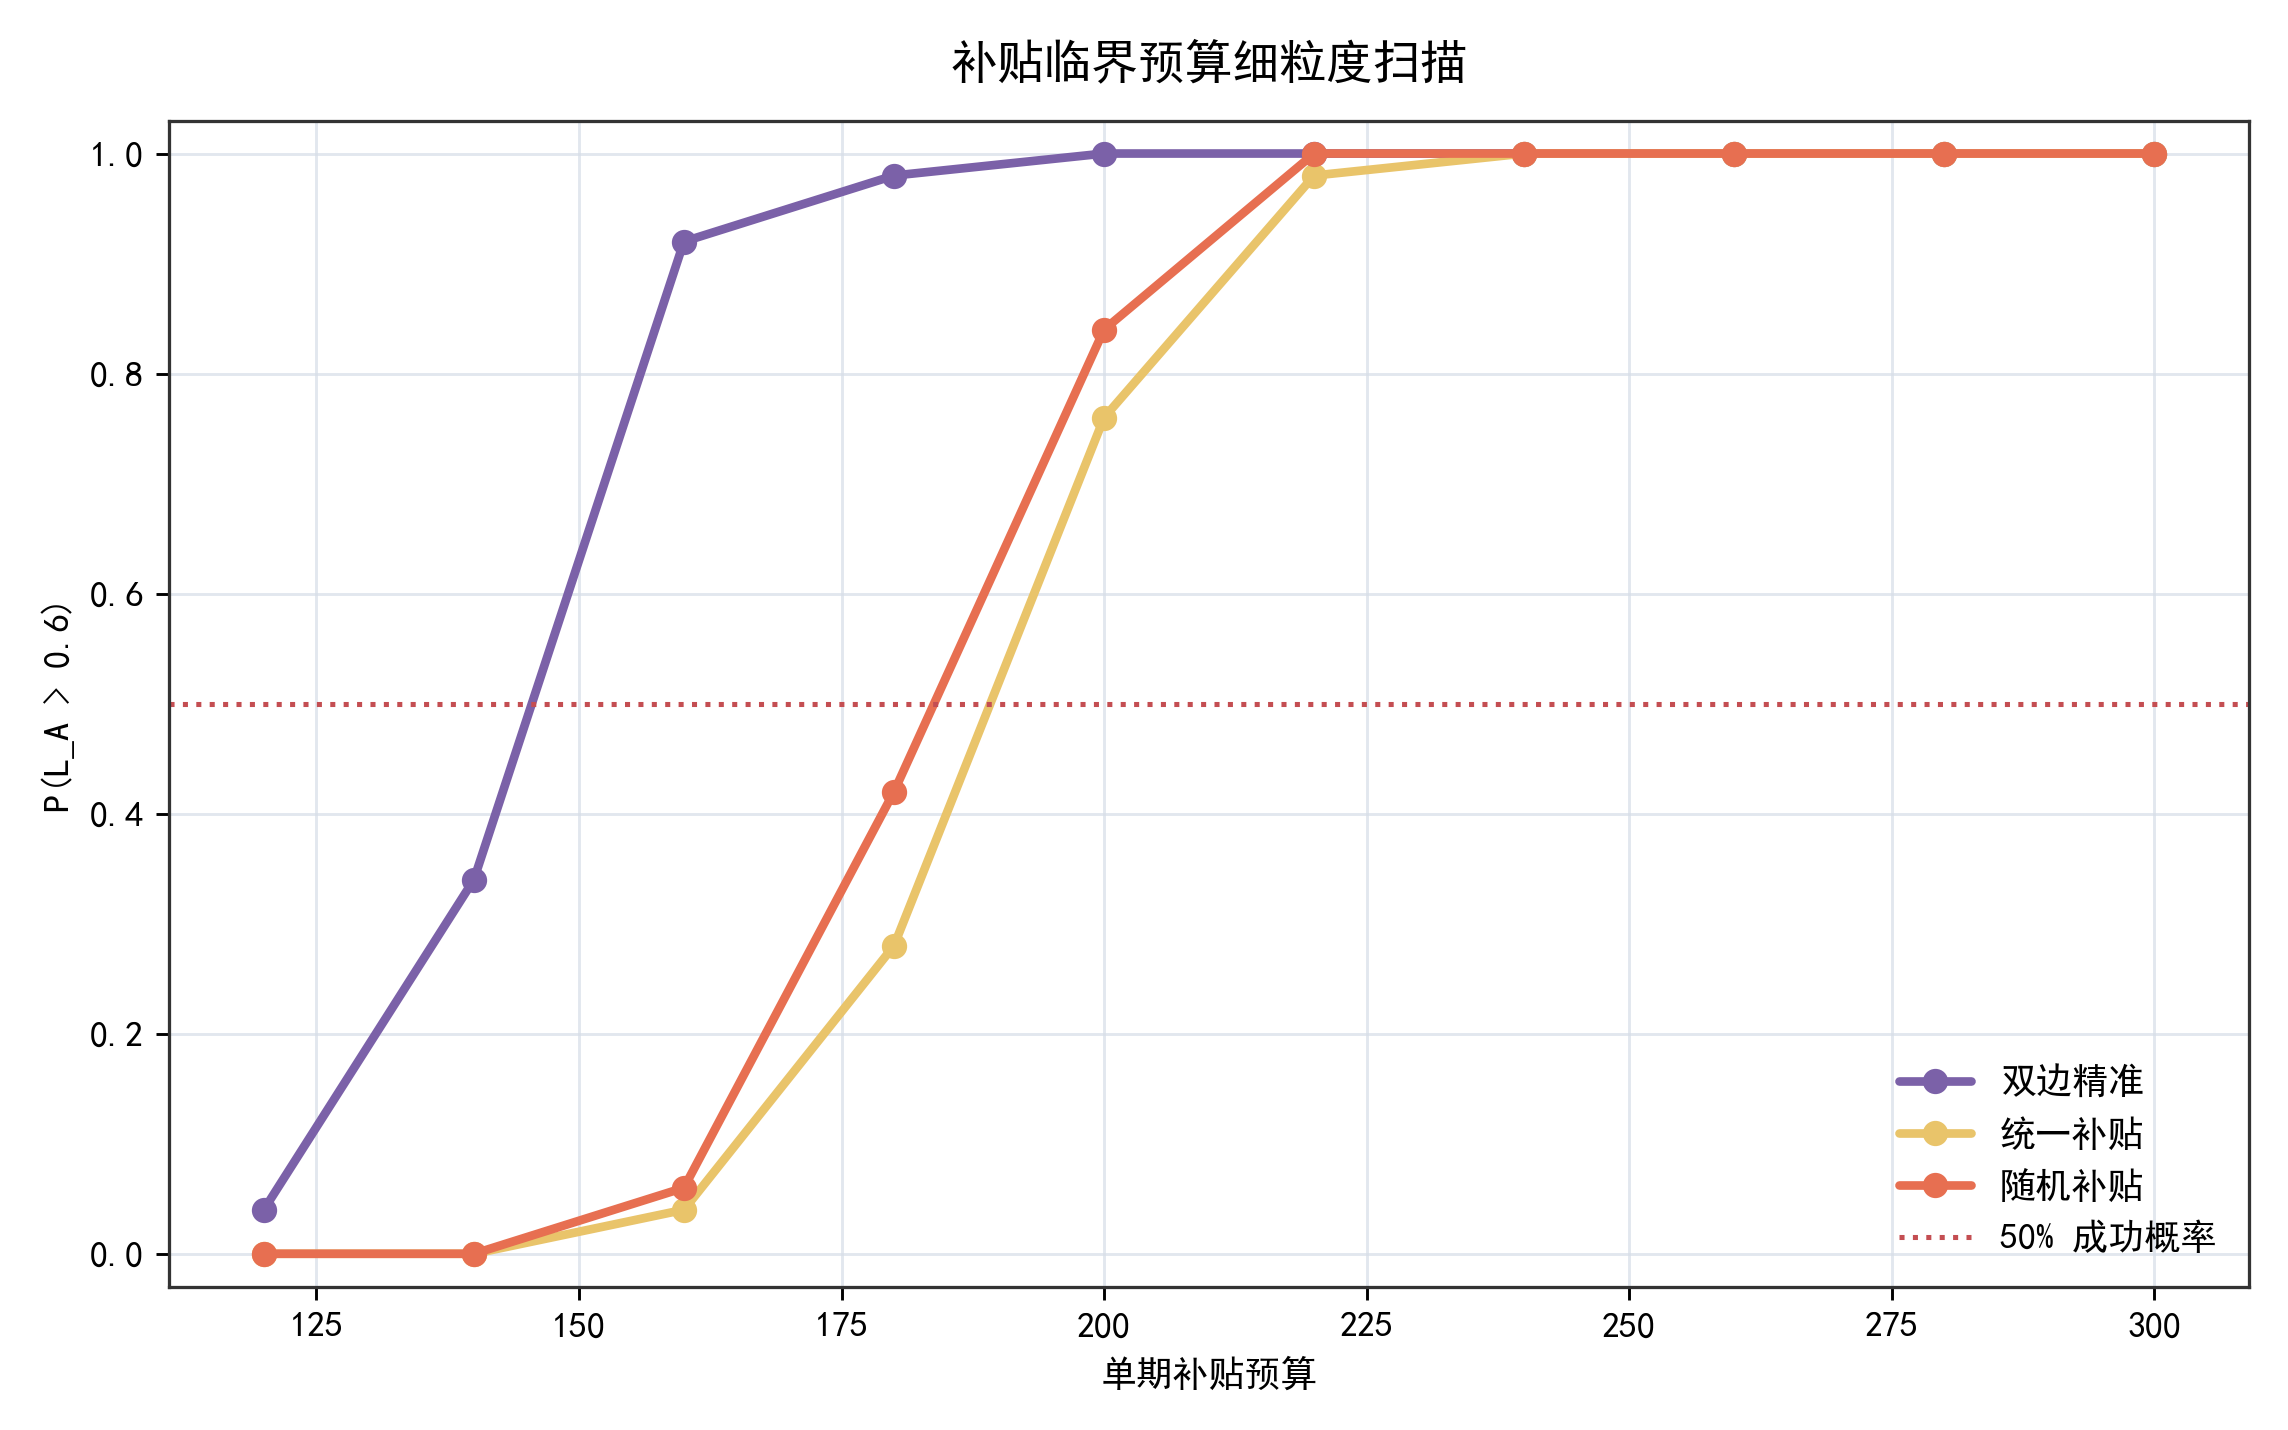
\includegraphics[width=\textwidth]{paper_B_budget_fine_success_curves.png}
    \caption{成功概率曲线}
  \end{subfigure}
  \hfill
  \begin{subfigure}{0.49\textwidth}
    \centering
    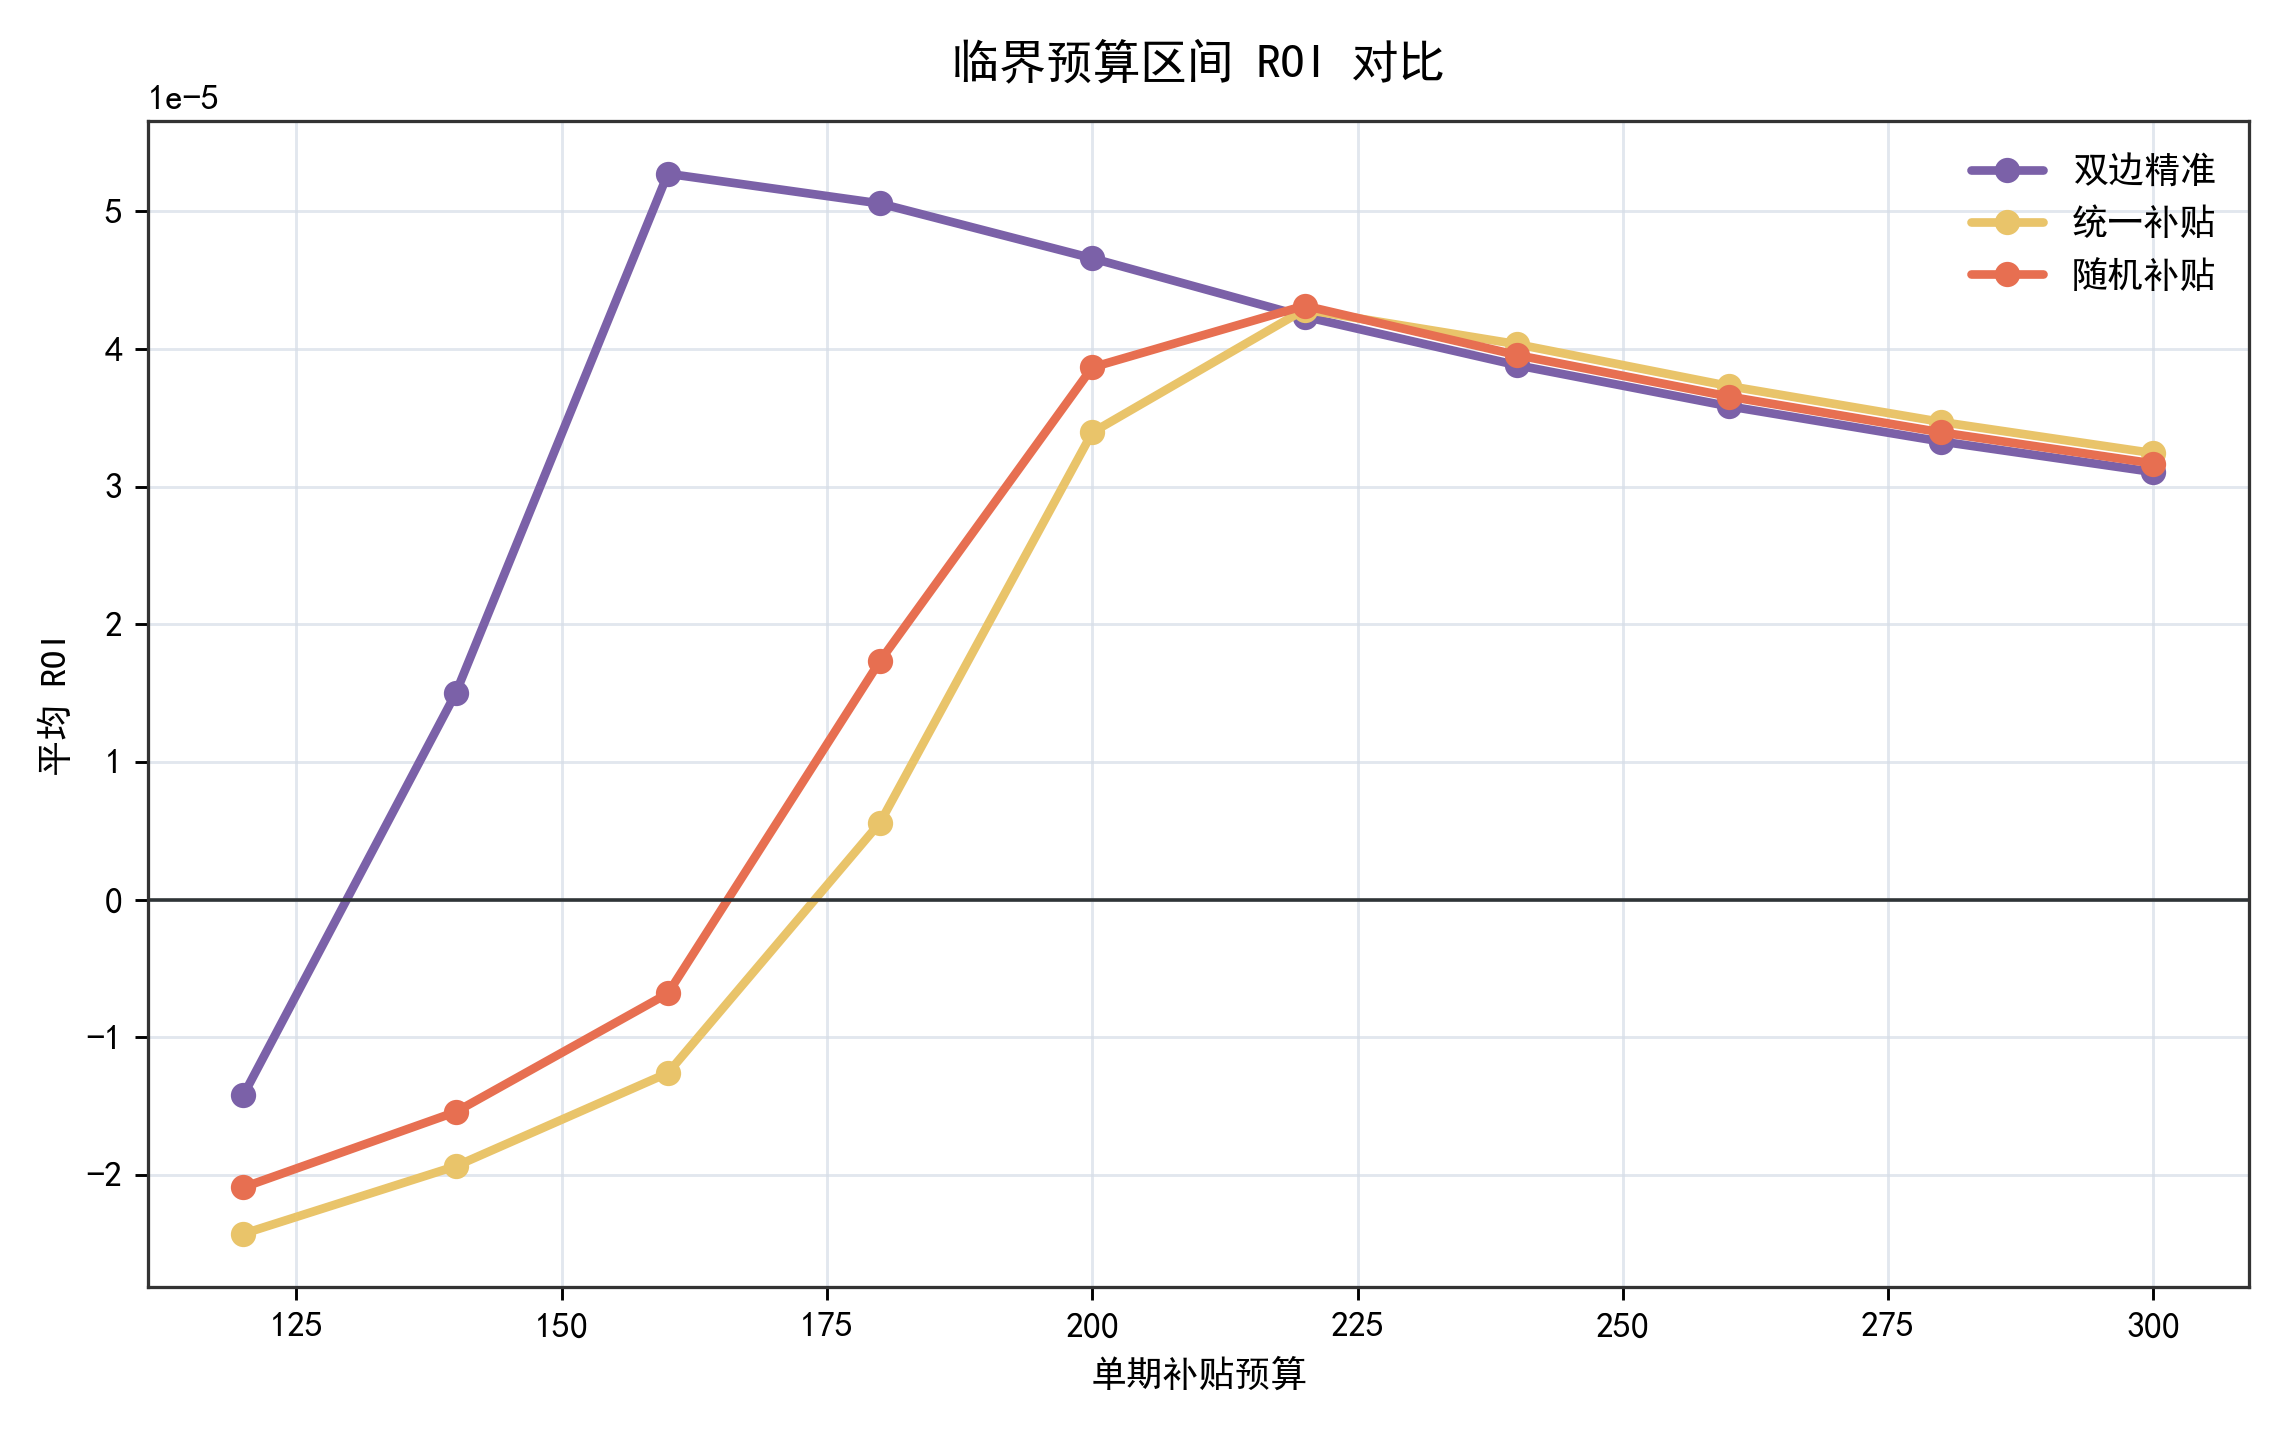
\includegraphics[width=\textwidth]{paper_B_budget_fine_roi_curves.png}
    \caption{ROI 曲线}
  \end{subfigure}
  \caption{临界预算区间的补贴策略比较}
  \label{fig:exp-b}
\end{figure}

\begin{table}[H]
\centering
\caption{不同补贴策略的临界预算估计}
\label{tab:budget-critical}
\begin{tabular}{lrrr}
\toprule
策略 & 临界预算 $B^*$ & 最大成功概率 & 最优 ROI \\
\midrule
统一补贴 & 200 & 1.00 & 0.000043 \\
随机补贴 & 200 & 1.00 & 0.000043 \\
双边精准 & 160 & 1.00 & 0.000053 \\
\bottomrule
\end{tabular}
\end{table}

\begin{table}[H]
\centering
\caption{细粒度预算扫描下的成功概率}
\label{tab:budget-prob}
\begin{tabular}{rrrr}
\toprule
预算 $B$ & 双边精准 & 统一补贴 & 随机补贴 \\
\midrule
120 & 0.04 & 0.00 & 0.00 \\
140 & 0.34 & 0.00 & 0.00 \\
160 & 0.92 & 0.04 & 0.06 \\
180 & 0.98 & 0.28 & 0.42 \\
200 & 1.00 & 0.76 & 0.84 \\
220 & 1.00 & 0.98 & 1.00 \\
240 & 1.00 & 1.00 & 1.00 \\
260 & 1.00 & 1.00 & 1.00 \\
280 & 1.00 & 1.00 & 1.00 \\
300 & 1.00 & 1.00 & 1.00 \\
\bottomrule
\end{tabular}
\end{table}

结果表明，补贴效果存在明显临界预算。双边精准补贴在 $B=160$ 时成功概率达到 0.92，而统一补贴和随机补贴在同一预算下成功概率分别只有 0.04 和 0.06。统一补贴与随机补贴的临界预算约为 200，双边精准补贴的临界预算约为 160，说明同时推动摇摆用户和关键商户可以将跨越临界规模所需预算降低约 20\%。ROI 曲线也显示，预算过高后所有有效策略都趋于成功，但边际收益下降，因此补贴最有价值的区间恰好位于临界规模附近。

\section{实验 C：冷启动二维资源配比}

\subsection{实验目的与设计}

冷启动实验关注新平台或弱势平台需要怎样的用户侧和商户侧初始资源组合，才能触发双边正反馈。细粒度实验扫描
\[
u_A(0),m_A(0)\in\{0.300,0.325,\ldots,0.500\},
\]
每个网格点重复运行 50 次。

\begin{figure}[H]
  \centering
  \begin{subfigure}{0.49\textwidth}
    \centering
    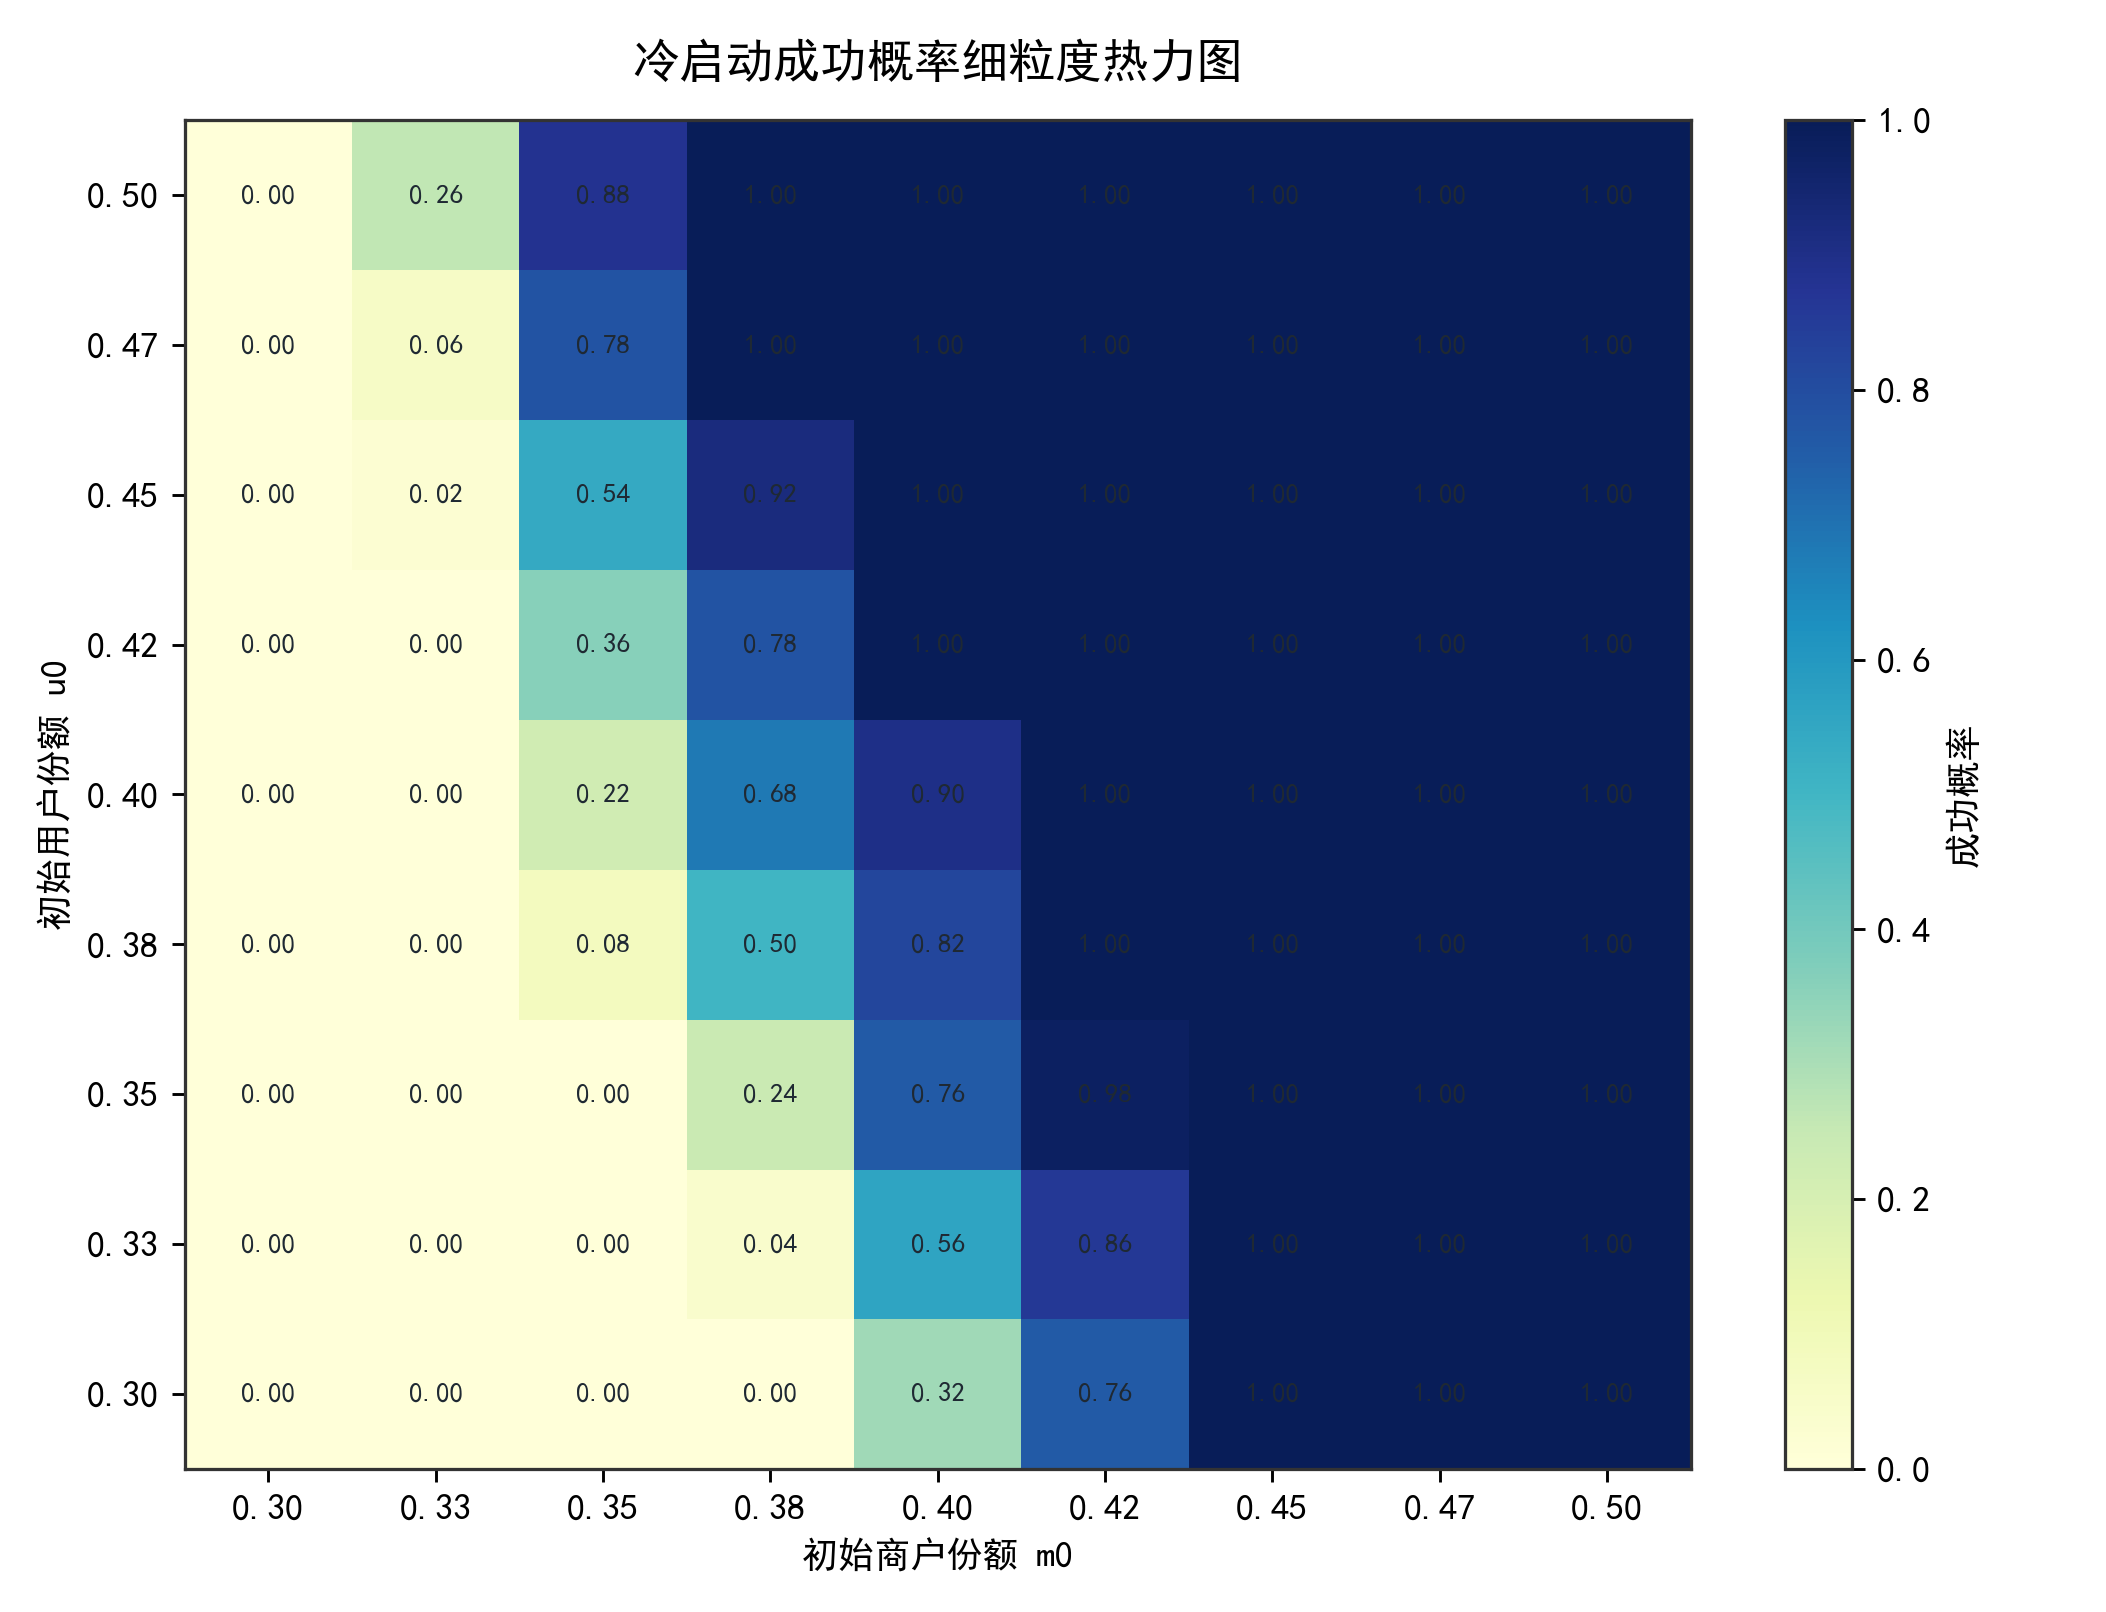
\includegraphics[width=\textwidth]{paper_C_cold_start_fine_success_heatmap.png}
    \caption{成功概率热力图}
  \end{subfigure}
  \hfill
  \begin{subfigure}{0.49\textwidth}
    \centering
    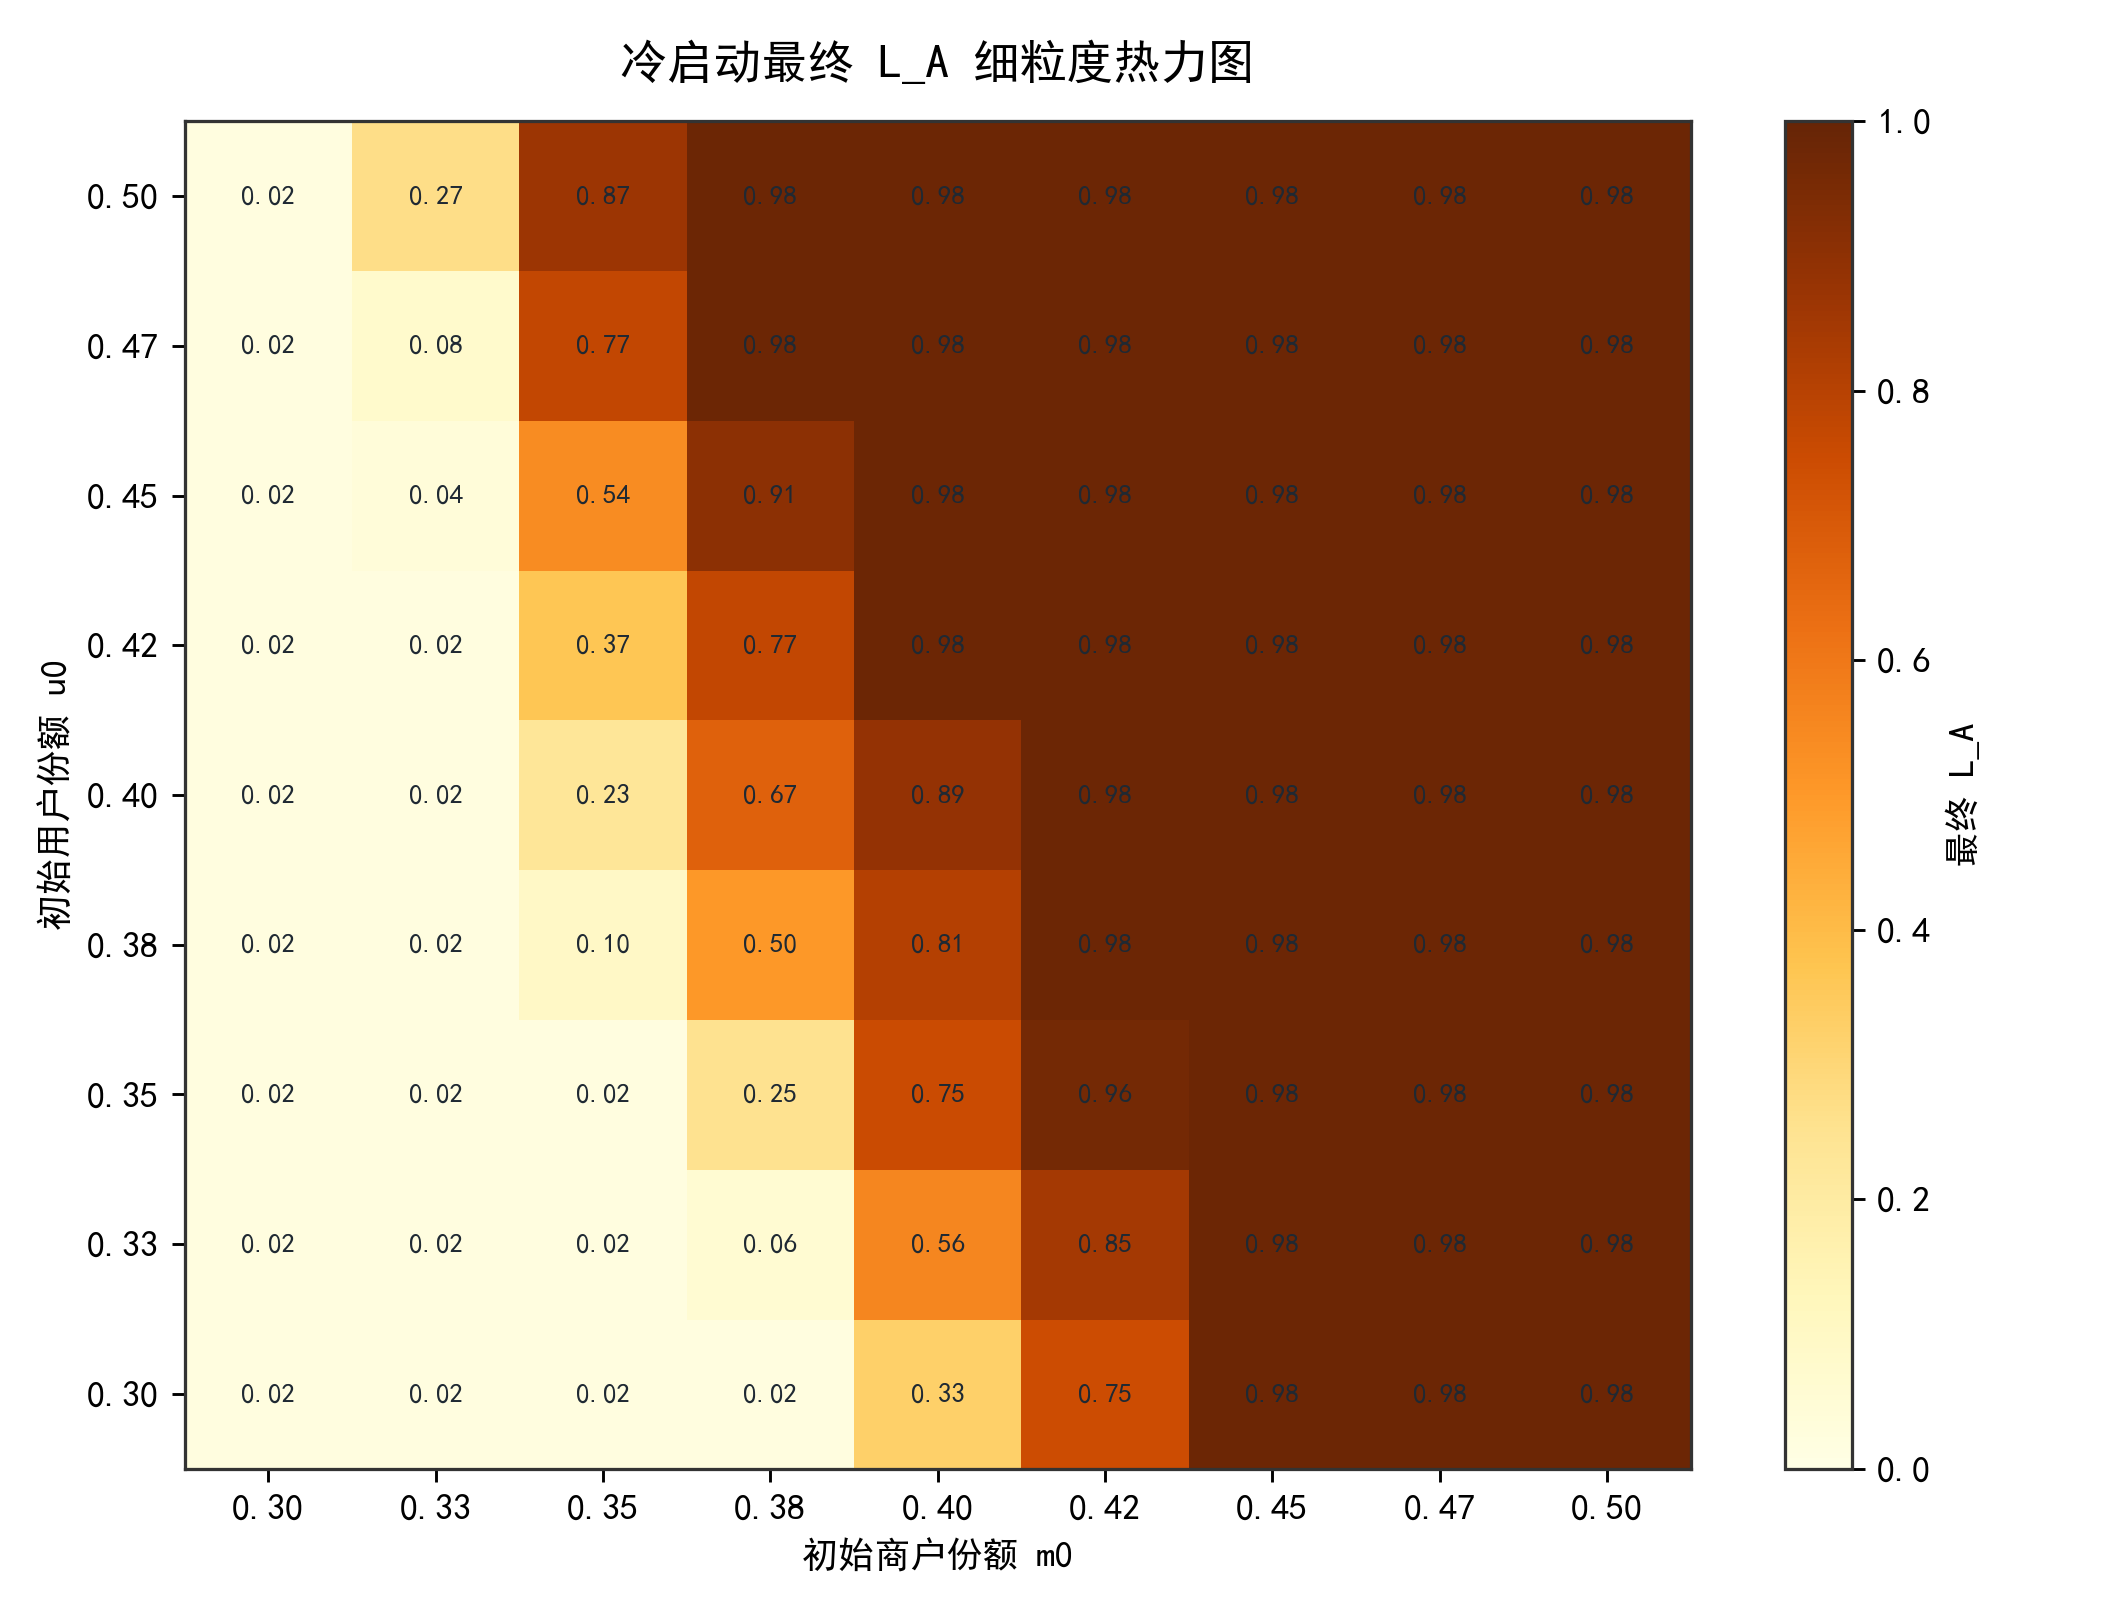
\includegraphics[width=\textwidth]{paper_C_cold_start_fine_final_L_heatmap.png}
    \caption{最终 $L_A$ 热力图}
  \end{subfigure}
  \caption{冷启动关键区域的细粒度扫描}
  \label{fig:exp-c}
\end{figure}

\begin{table}[H]
\centering
\caption{冷启动边界附近的成功概率示例}
\label{tab:cold-start}
\begin{tabular}{rrrrrrrr}
\toprule
\multirow{2}{*}{$m_A(0)$} & \multicolumn{7}{c}{$u_A(0)$} \\
\cmidrule(lr){2-8}
 & 0.325 & 0.350 & 0.375 & 0.400 & 0.425 & 0.450 & 0.475 \\
\midrule
0.325 & 0.00 & 0.00 & 0.00 & 0.00 & 0.00 & 0.02 & 0.06 \\
0.350 & 0.00 & 0.00 & 0.08 & 0.22 & 0.36 & 0.54 & 0.78 \\
0.375 & 0.04 & 0.24 & 0.50 & 0.68 & 0.78 & 0.92 & 1.00 \\
0.400 & 0.56 & 0.76 & 0.82 & 0.90 & 1.00 & 1.00 & 1.00 \\
0.425 & 0.86 & 0.98 & 1.00 & 1.00 & 1.00 & 1.00 & 1.00 \\
\bottomrule
\end{tabular}
\end{table}

图 \ref{fig:exp-c} 显示，冷启动成功区域主要位于右上方，但边界并非简单直线。当商户初始份额低于 0.35 时，提高用户初始份额的边际作用有限；当商户初始份额达到 0.375--0.425 时，用户侧资源的边际作用明显增强；当商户初始份额超过 0.45 后，平台基本进入稳定成功区。这说明供给侧资源在冷启动中具有底座作用，用户增长只有在商户供给达到一定水平后才能有效触发正反馈。

\begin{figure}[H]
  \centering
  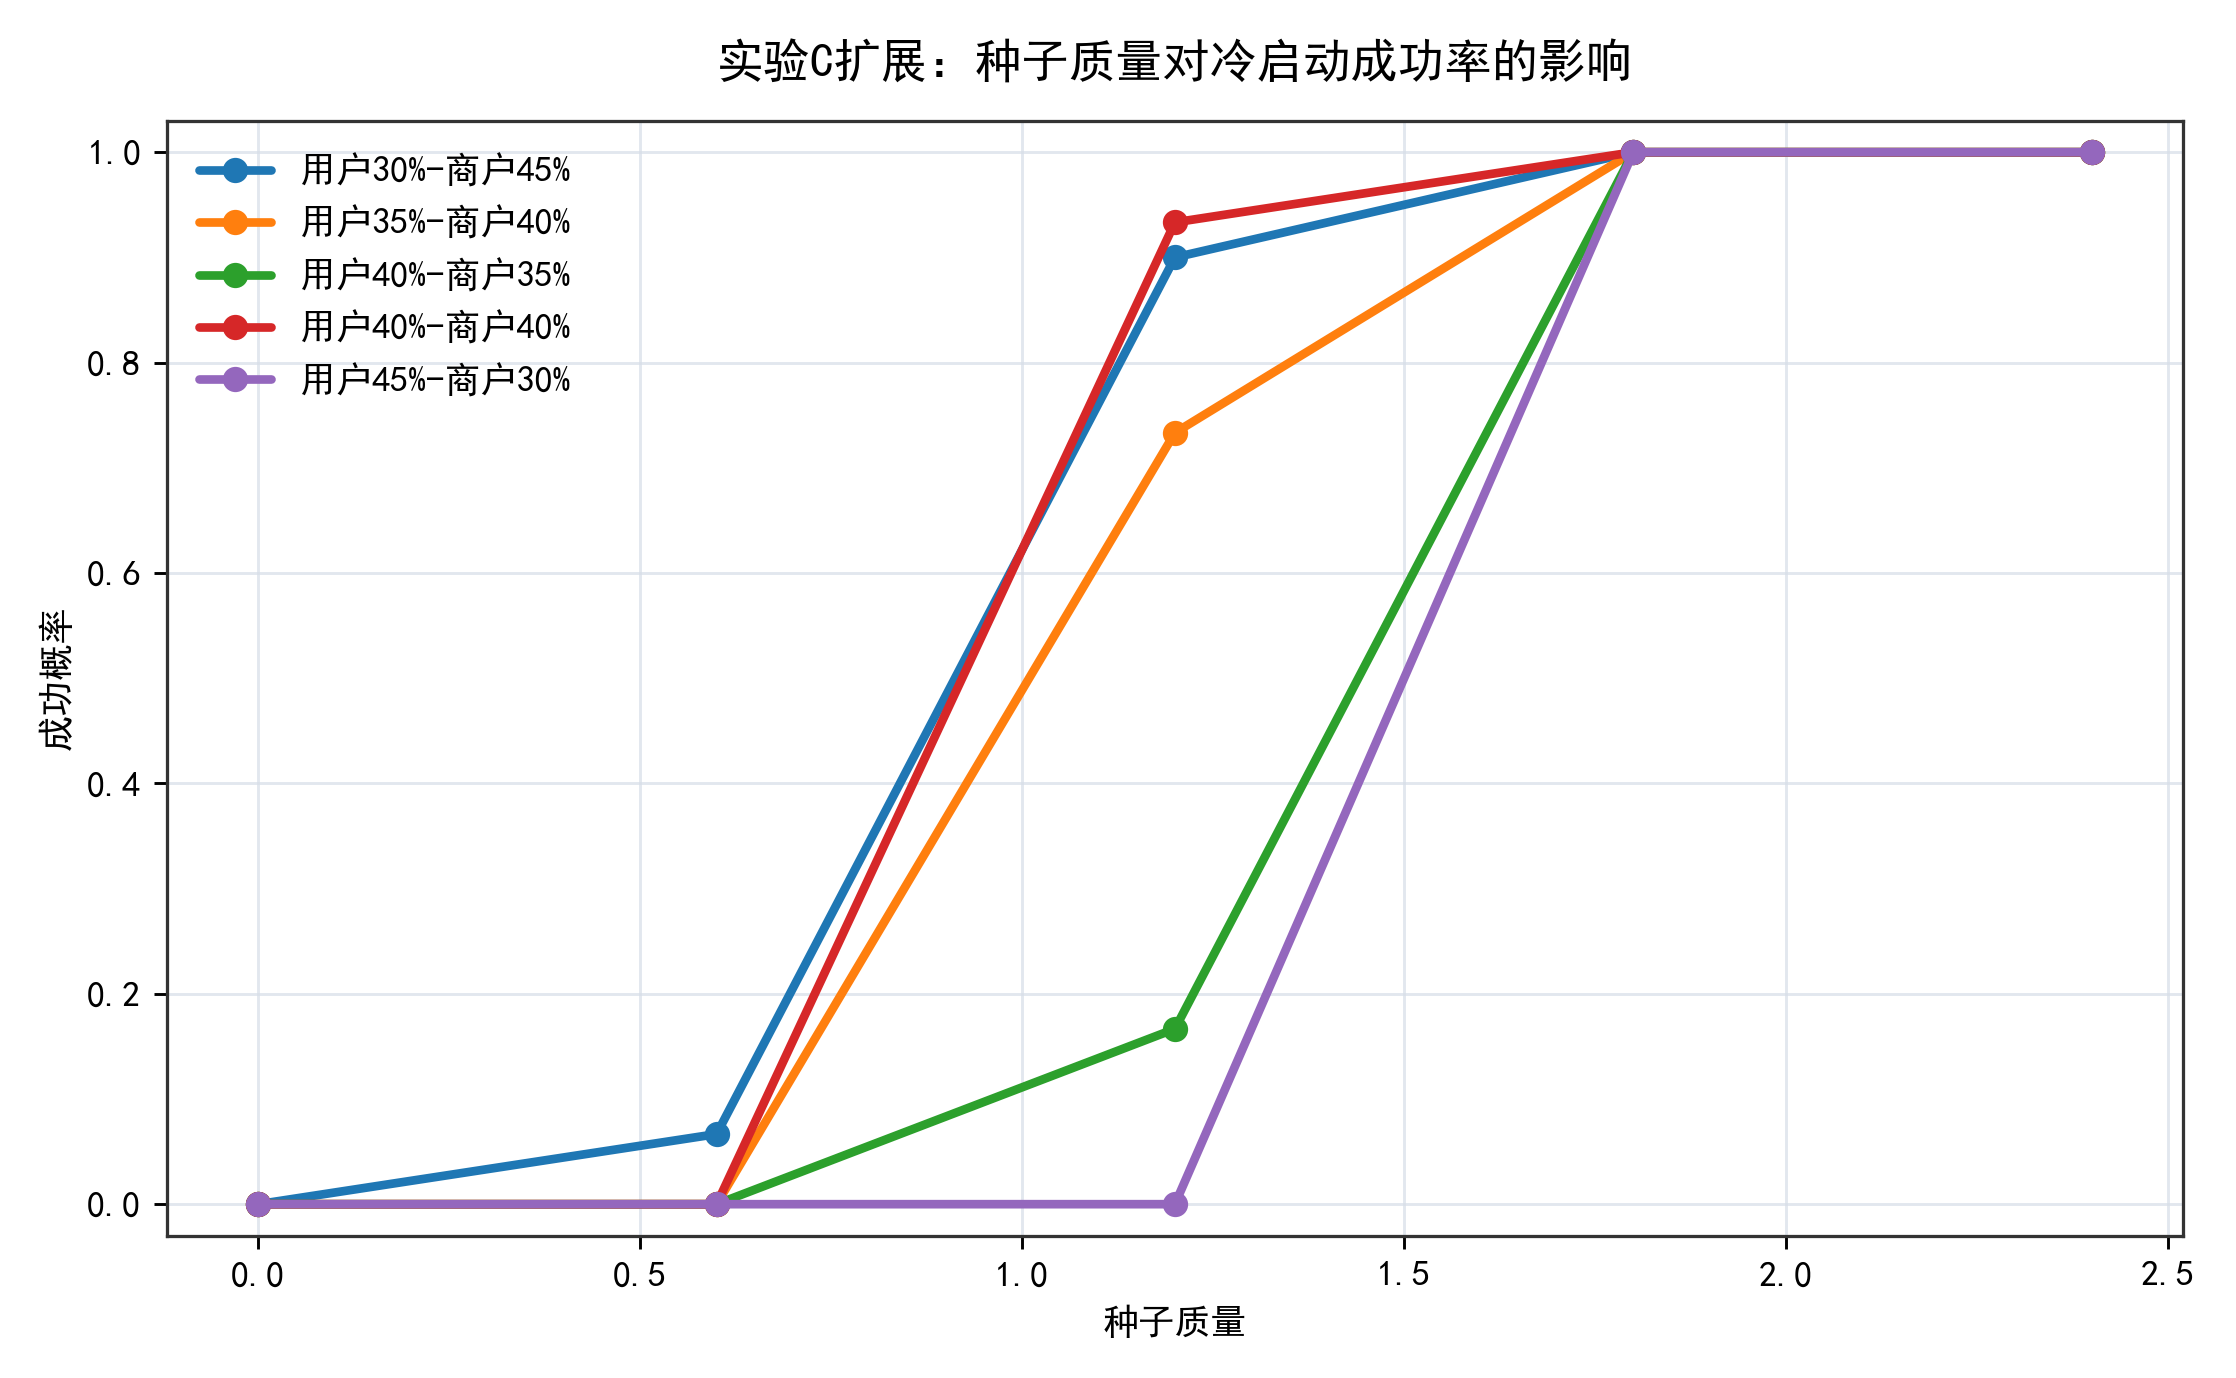
\includegraphics[width=0.78\textwidth]{revised_C_seed_quality_success_curves.png}
  \caption{种子质量对冷启动成功率的影响}
  \label{fig:seed-quality}
\end{figure}

种子质量实验进一步说明，冷启动不仅取决于种子数量，也取决于种子黏性和质量。在“用户 30\%--商户 45\%”组合中，种子质量为 0 时成功概率为 0，提高到 1.2 后成功概率升至 0.90，提高到 1.8 后达到 1.00。这表明平台可以通过签约、定向扶持、排他合作或服务承诺提高早期主体黏性，从而降低所需初始规模。

\section{实验 D：商户多归属成本阈值}

\subsection{实验目的与设计}

本实验考察多归属成本 $k_M$ 和多归属有效供给贡献 $\rho$ 如何影响平台共存。细粒度扫描设定为
\[
k_M\in\{0,0.05,0.10,0.15,0.20,0.30,0.40,0.50\},
\]
\[
\rho\in\{0.30,0.40,0.50,0.60,0.70\},
\]
每个参数组合重复 50 次。

\begin{figure}[H]
  \centering
  \begin{subfigure}{0.49\textwidth}
    \centering
    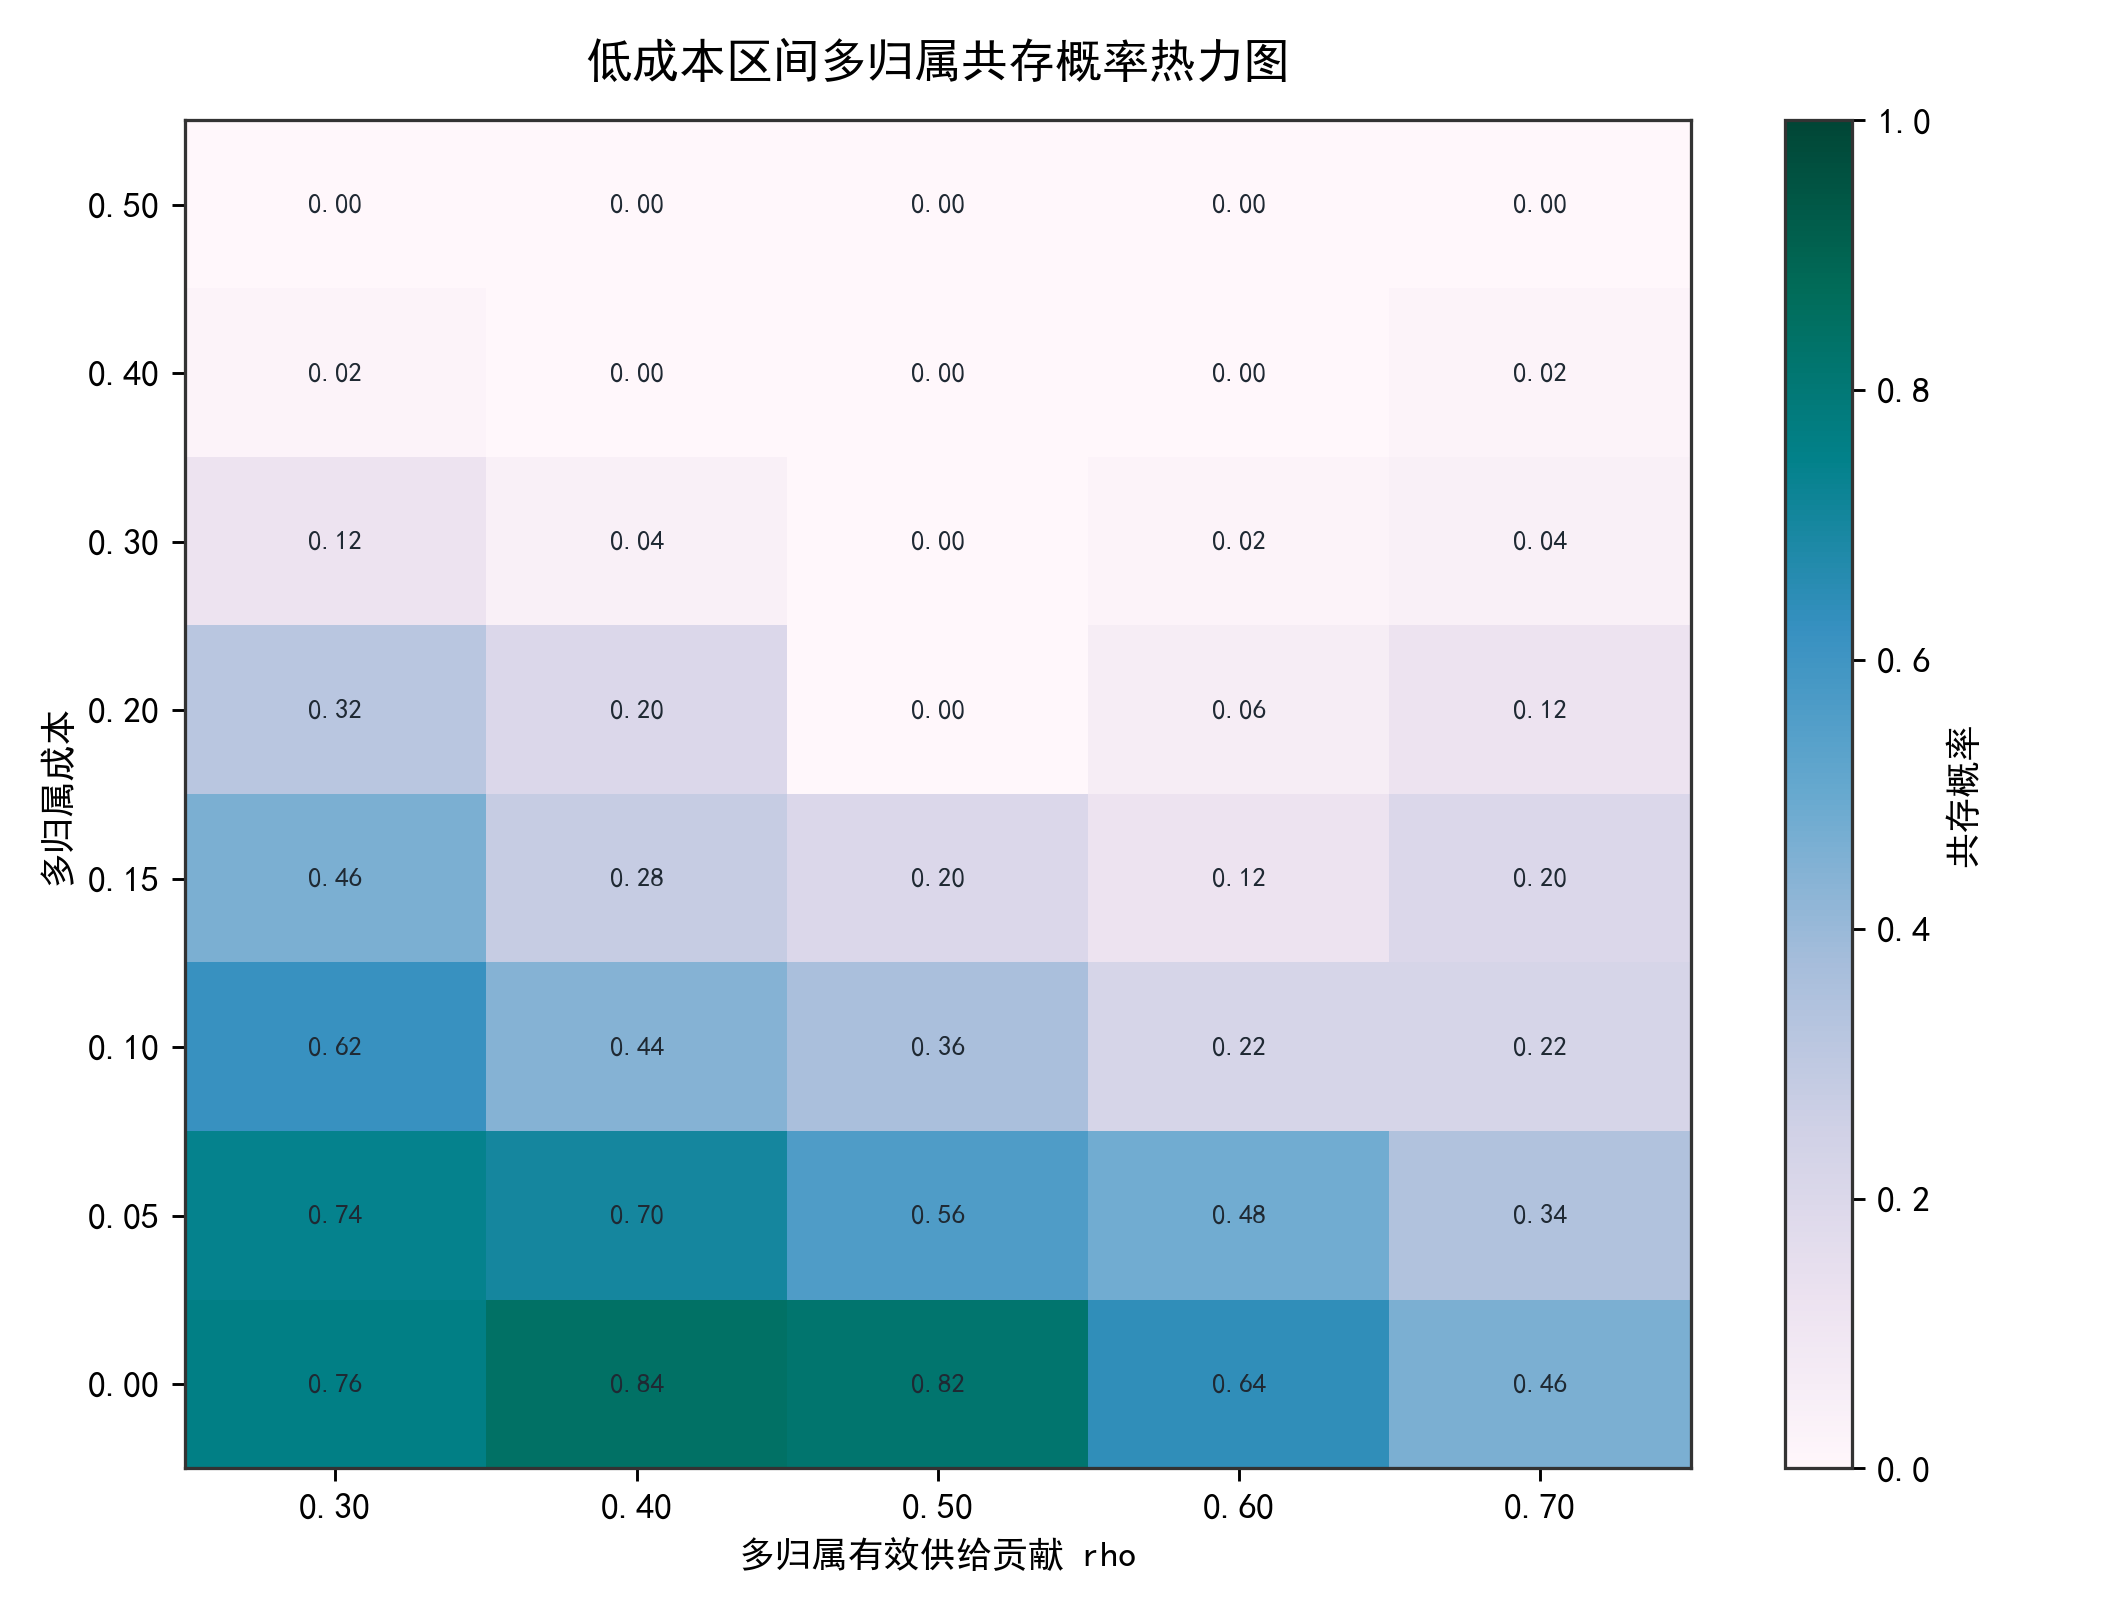
\includegraphics[width=\textwidth]{paper_D_multi_home_fine_coexist_heatmap.png}
    \caption{共存概率}
  \end{subfigure}
  \hfill
  \begin{subfigure}{0.49\textwidth}
    \centering
    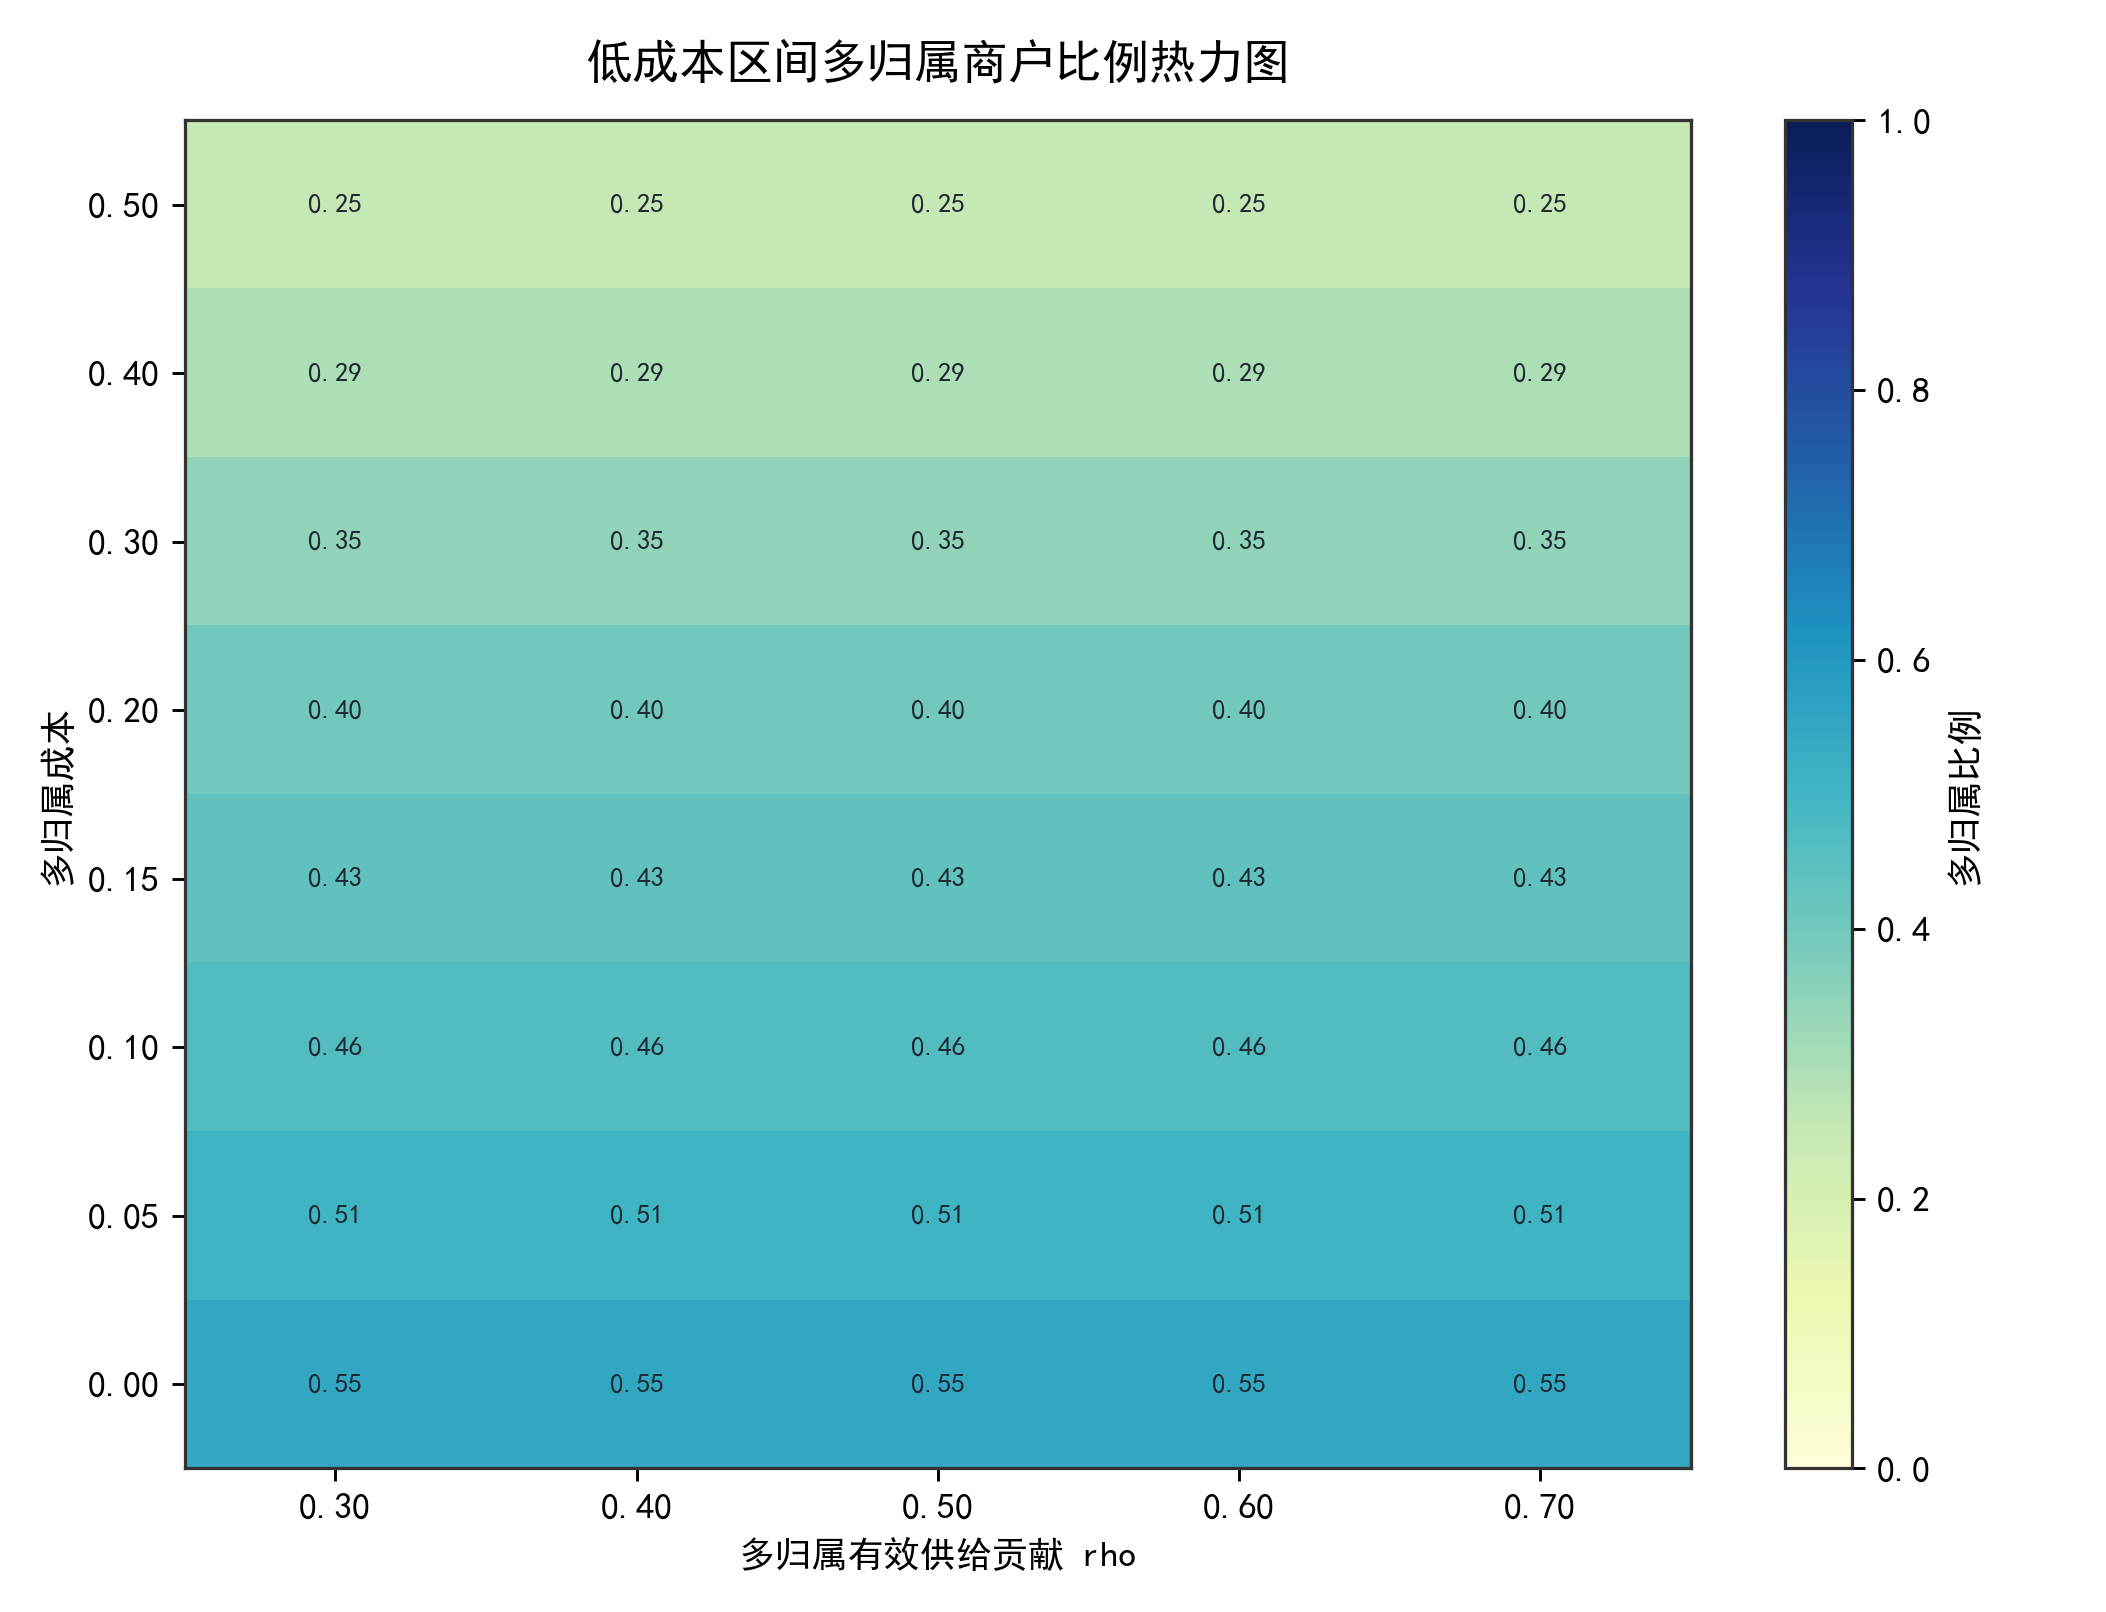
\includegraphics[width=\textwidth]{paper_D_multi_home_fine_share_heatmap.png}
    \caption{多归属商户比例}
  \end{subfigure}
  \caption{低成本区间多归属机制的细粒度扫描}
  \label{fig:exp-d}
\end{figure}

\begin{table}[H]
\centering
\caption{低成本区间的共存概率}
\label{tab:multi-home}
\begin{tabular}{rrrrrr}
\toprule
$k_M$ & $\rho=0.30$ & $\rho=0.40$ & $\rho=0.50$ & $\rho=0.60$ & $\rho=0.70$ \\
\midrule
0.00 & 0.76 & 0.84 & 0.82 & 0.64 & 0.46 \\
0.05 & 0.74 & 0.70 & 0.56 & 0.48 & 0.34 \\
0.10 & 0.62 & 0.44 & 0.36 & 0.22 & 0.22 \\
0.15 & 0.46 & 0.28 & 0.20 & 0.12 & 0.20 \\
0.20 & 0.32 & 0.20 & 0.00 & 0.06 & 0.12 \\
0.30 & 0.12 & 0.04 & 0.00 & 0.02 & 0.04 \\
0.40 & 0.02 & 0.00 & 0.00 & 0.00 & 0.02 \\
0.50 & 0.00 & 0.00 & 0.00 & 0.00 & 0.00 \\
\bottomrule
\end{tabular}
\end{table}

结果显示，多归属成本是平台共存的重要约束。$k_M=0$ 时，共存概率最高可达 0.84；当成本上升到 0.20 后，共存概率明显下降；当成本达到 0.50 时，共存概率几乎为 0。与此同时，$\rho$ 的作用不是简单单调的。较高 $\rho$ 虽然提高多归属商户对两侧平台的有效供给，但在存在初始优势时，也可能使优势平台更快积累用户吸引力，从而降低共存概率。

\begin{figure}[H]
  \centering
  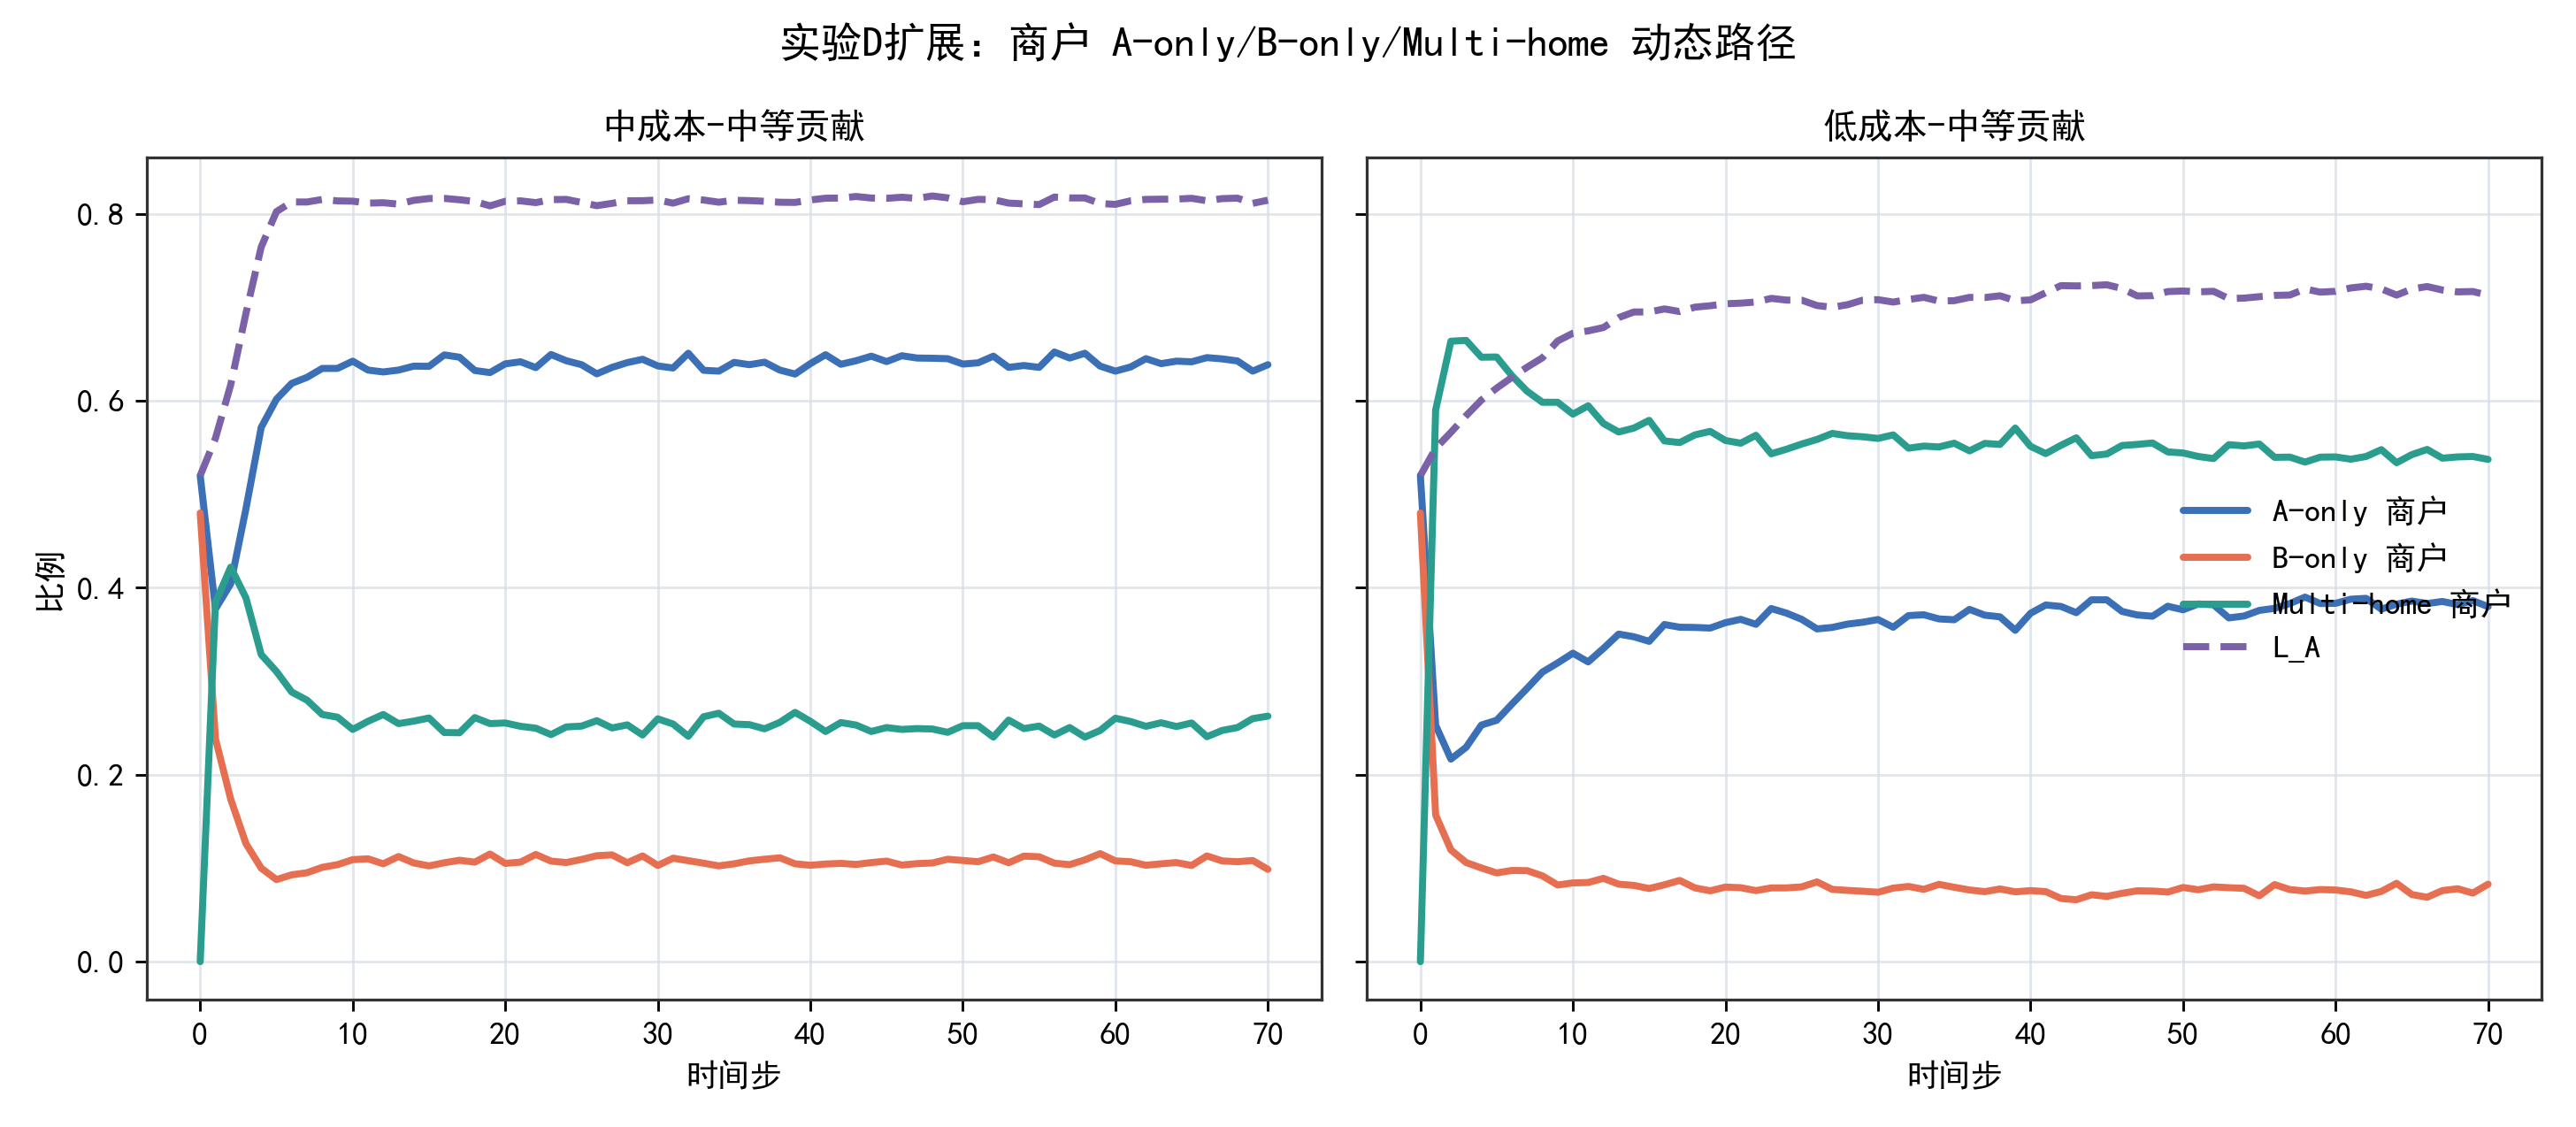
\includegraphics[width=0.88\textwidth]{revised_D_multi_home_state_paths.png}
  \caption{A-only、B-only 与 multi-home 商户状态的动态路径}
  \label{fig:multi-path}
\end{figure}

动态路径显示，低成本场景下 multi-home 商户可长期保持较高比例，从而缓和平台间供给差异；高成本场景中，商户迅速收敛到单一平台，市场更容易走向锁定。这说明多归属政策不仅改变最终状态，也改变竞争过程中的供给迁移速度。

\section{实验 E：机制消融}

\subsection{实验目的与设计}

前述实验给出了补贴、冷启动和多归属机制下的结果，但仍需回答一个关键问题：这些结果究竟来自哪个机制？因此，本实验在补贴临界区设置消融对照。基准版本保留个体异质性、惯性、双边网络效应、双边精准补贴和商户多归属；随后逐一去掉某一机制，比较平台 A 的成功概率、A 锁定概率和最终 $L_A$。

实验设定为
\[
u_A(0)=0.30,\qquad m_A(0)=0.30,\qquad B=140,
\]
网络效应为 $\alpha=\beta=2.5$，每个版本重复运行 30 次。该设定位于弱势平台跨越临界规模的敏感区域，因而适合观察关键机制被移除后的结果变化。

\begin{figure}[H]
  \centering
  \begin{subfigure}{0.49\textwidth}
    \centering
    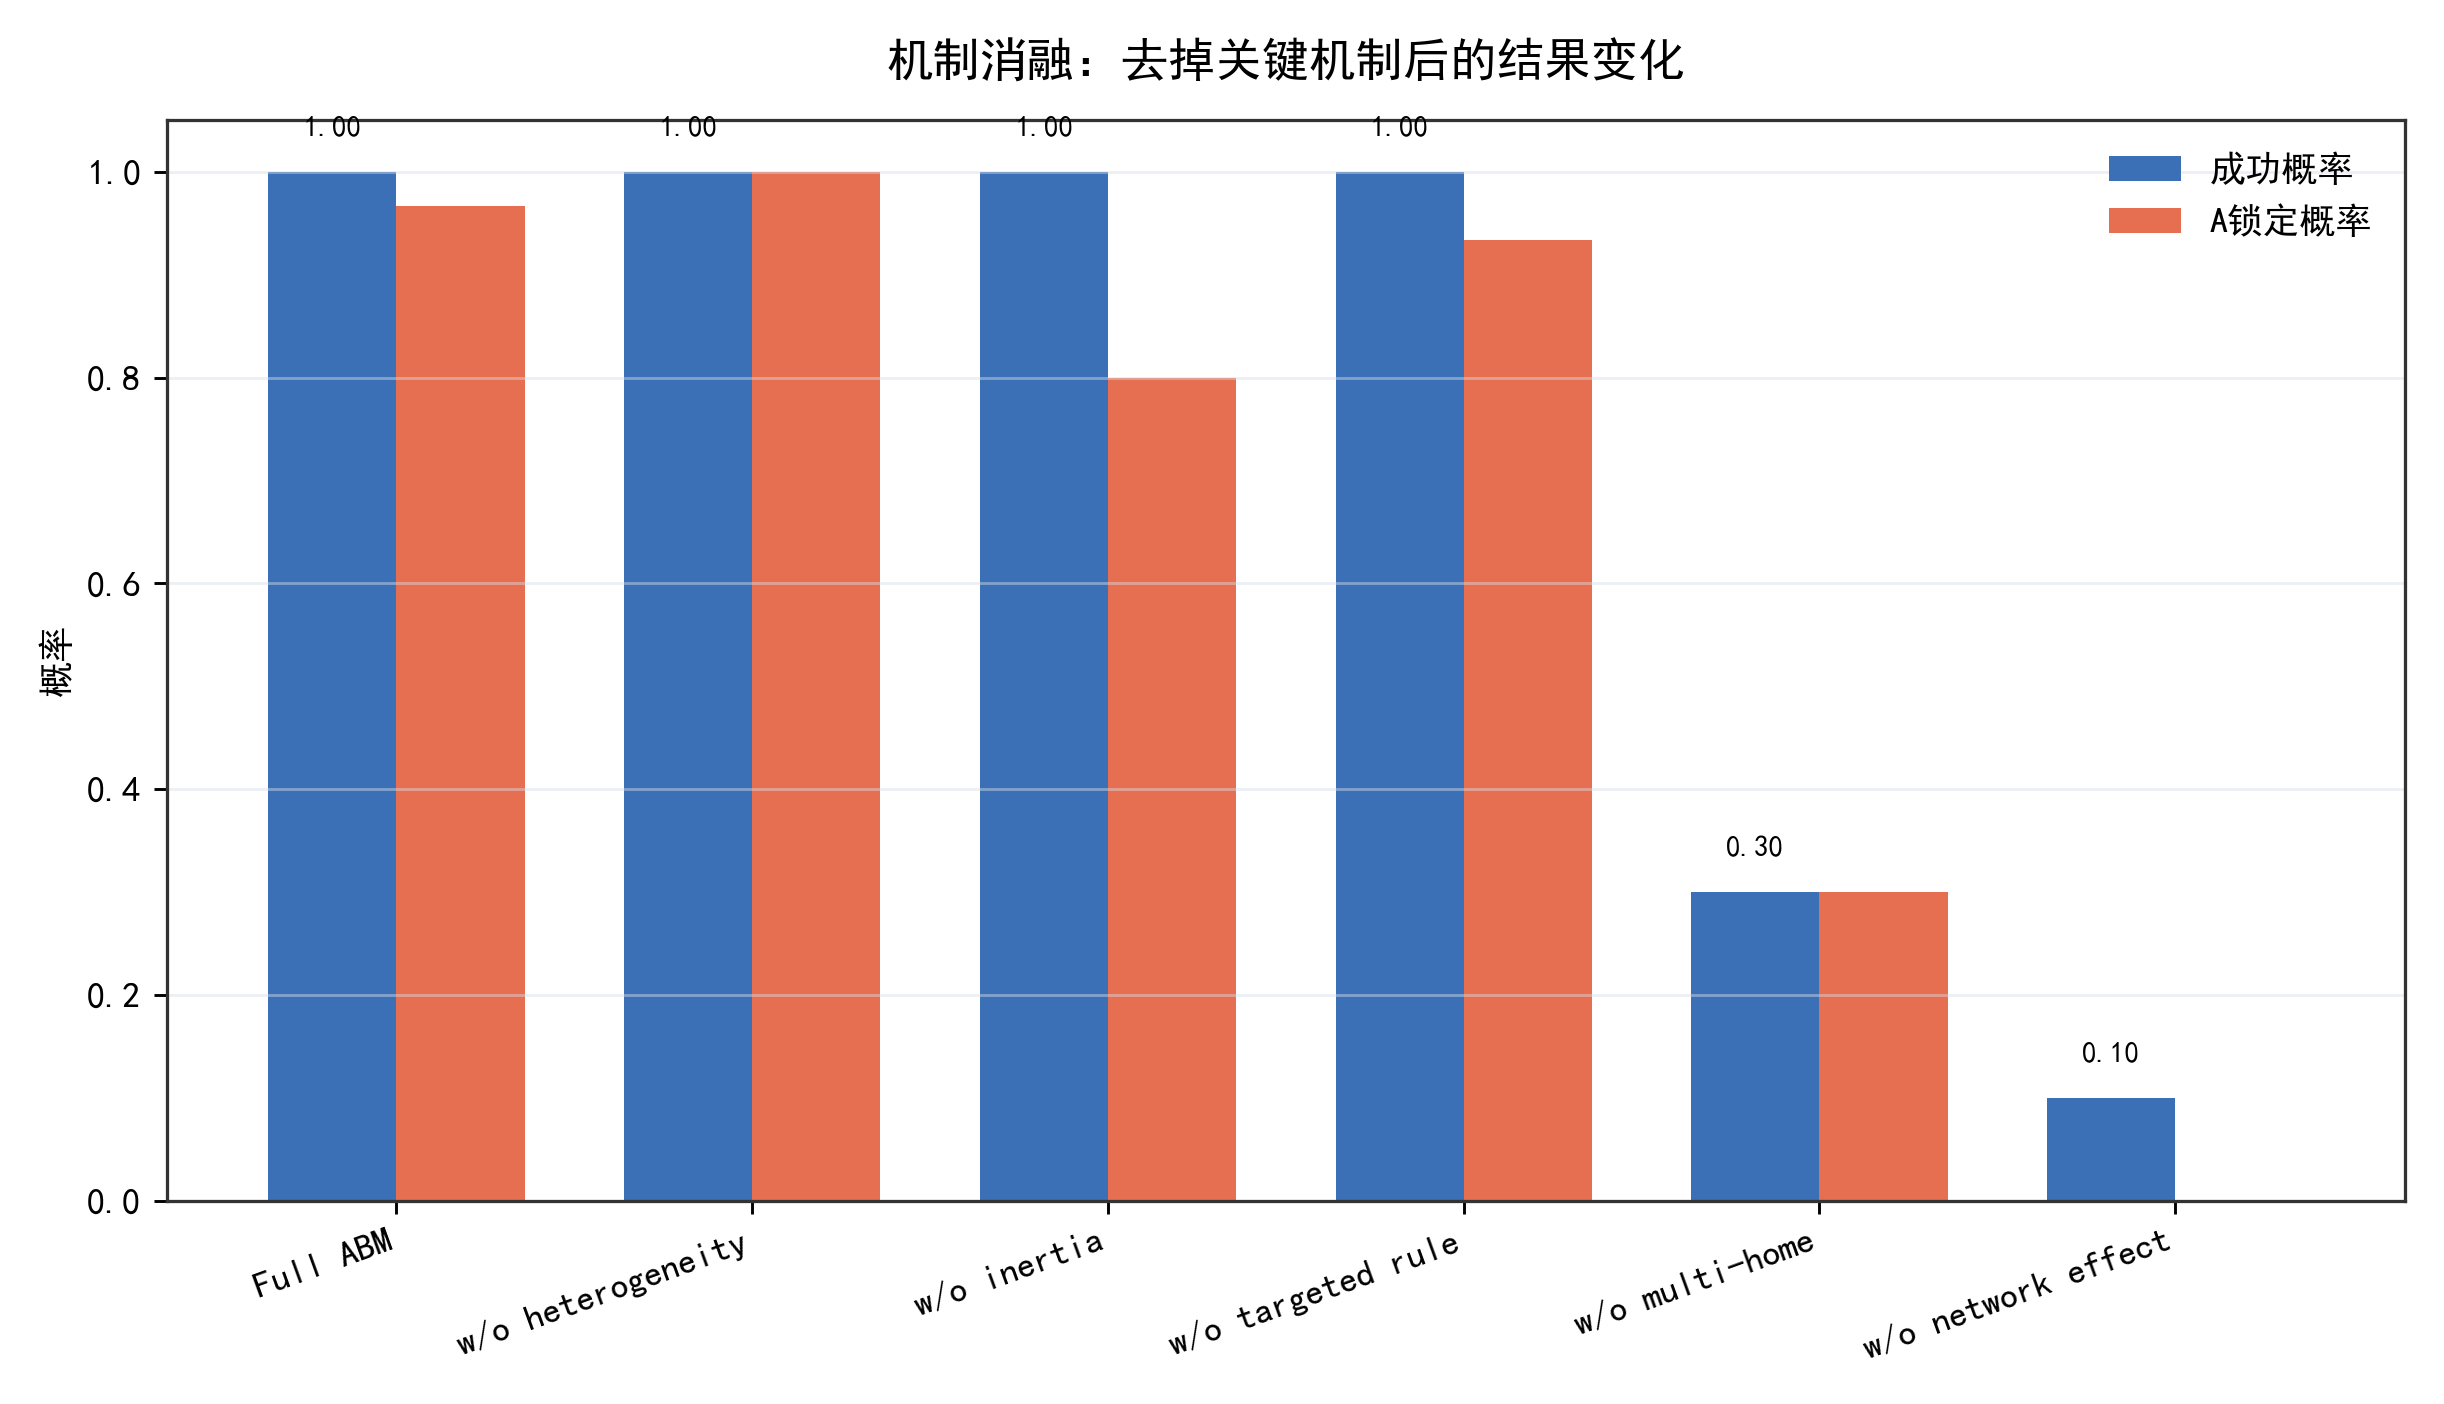
\includegraphics[width=\textwidth]{abm_mechanism_ablation_probabilities.png}
    \caption{成功概率与 A 锁定概率}
  \end{subfigure}
  \hfill
  \begin{subfigure}{0.49\textwidth}
    \centering
    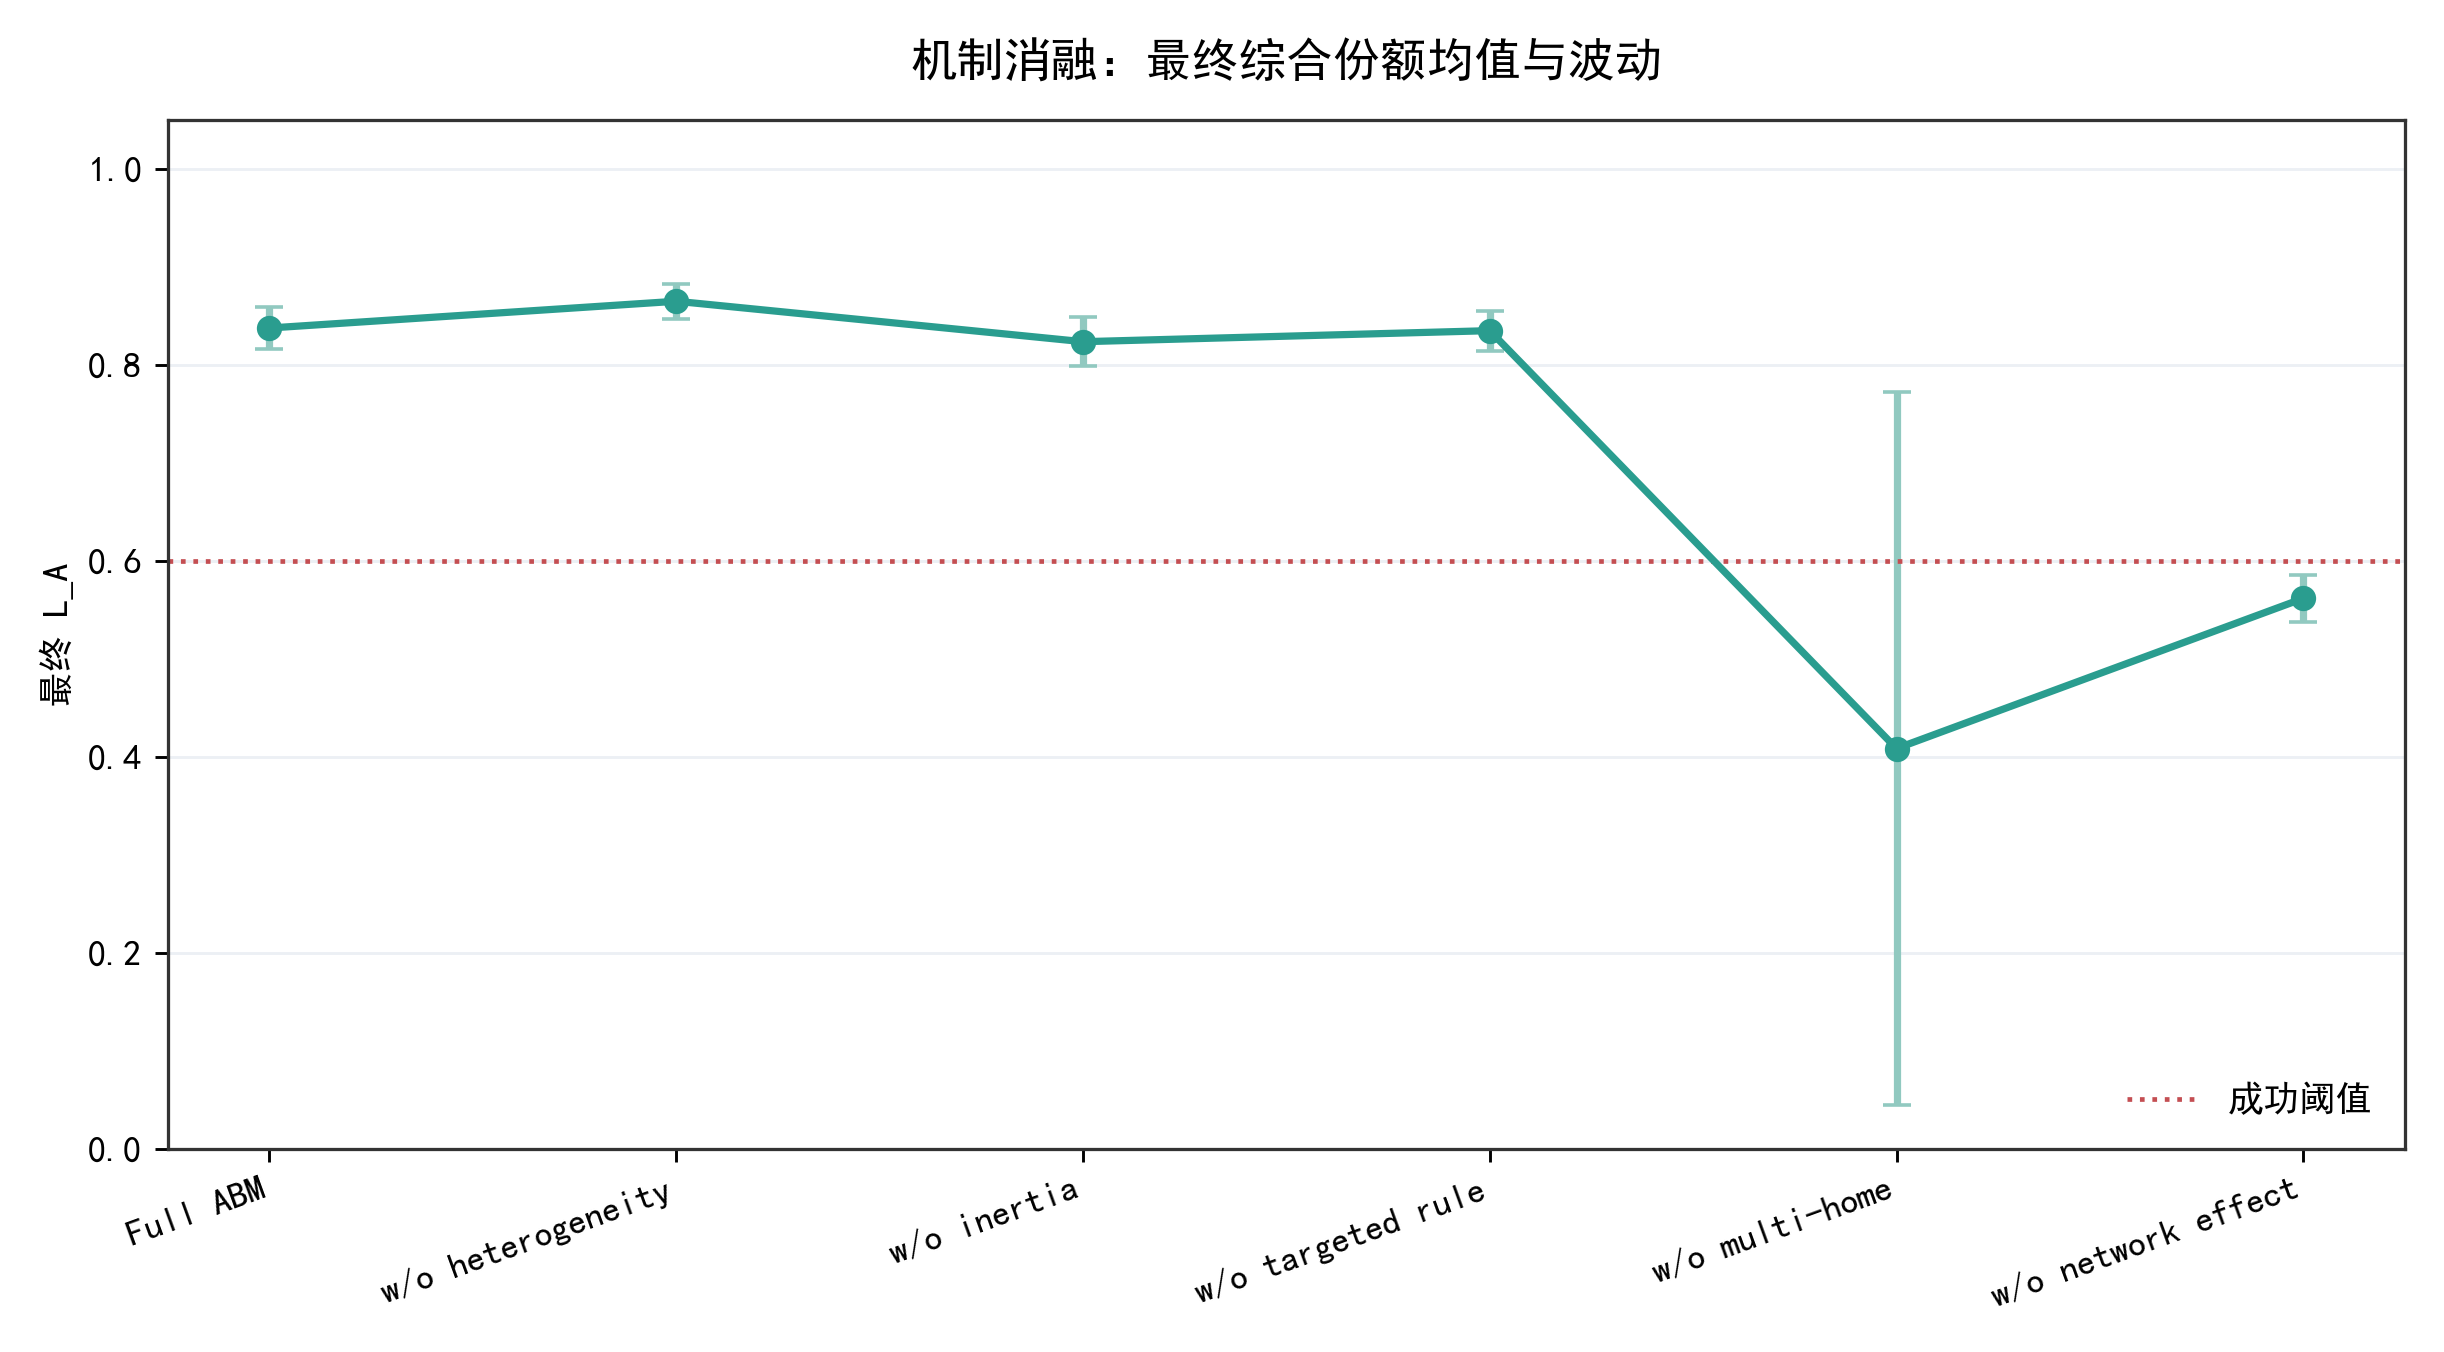
\includegraphics[width=\textwidth]{abm_mechanism_ablation_final_L.png}
    \caption{最终 $L_A$ 均值与标准差}
  \end{subfigure}
  \caption{机制消融实验结果}
  \label{fig:ablation}
\end{figure}

\begin{table}[H]
\centering
\caption{机制消融结果}
\label{tab:ablation}
\begin{tabular}{lrrrr}
\toprule
模型版本 & $\bar L_A$ & $sd(L_A)$ & 成功概率 & A 锁定概率 \\
\midrule
Full ABM & 0.838 & 0.022 & 1.000 & 0.967 \\
w/o heterogeneity & 0.865 & 0.018 & 1.000 & 1.000 \\
w/o inertia & 0.824 & 0.025 & 1.000 & 0.800 \\
w/o targeted rule & 0.835 & 0.021 & 1.000 & 0.933 \\
w/o multi-home & 0.409 & 0.364 & 0.300 & 0.300 \\
w/o network effect & 0.562 & 0.024 & 0.100 & 0.000 \\
\bottomrule
\end{tabular}
\end{table}

消融结果表明，双边网络效应是平台跨越临界规模的基础机制。去掉网络效应后，最终 $L_A$ 均值仅为 0.562，成功概率降至 0.100，且 A 锁定概率为 0。这说明补贴本身并不能独立产生稳定锁定，必须通过用户侧和商户侧的交叉反馈被放大。

多归属机制同样重要。去掉商户多归属后，成功概率从 1.000 降至 0.300，最终 $L_A$ 的标准差升至 0.364，说明多归属在弱势平台启动阶段具有缓冲作用：它降低供给侧排他性，使平台 A 在仍处劣势时也能获得一定有效供给，从而提高跨越临界区的机会。

惯性机制主要影响锁定强度而非是否成功。去掉惯性后，成功概率仍为 1.000，但 A 锁定概率从 0.967 降至 0.800，共存概率上升。这意味着惯性和切换成本并不是平台获得初步优势的唯一来源，但会强化路径依赖，使优势更容易固化为锁定。相比之下，将精准补贴改为随机补贴在本组参数下只使 A 锁定概率从 0.967 降至 0.933，说明当网络效应和多归属条件已经足以帮助平台接近临界规模时，补贴识别规则的边际贡献会被部分削弱；结合实验 B 可知，精准补贴的价值主要体现在预算更紧、平台尚未接近临界规模的区间。

\section{实验 F：ABM 与 ODE 结果对比}

\subsection{实验目的与设计}

为了明确 ABM 与宏观 ODE 模型之间的关系，本实验选取三类代表性场景进行对比：弱网络效应、强网络效应和冷启动临界区。ODE 给出平均场轨迹；ABM 在相同宏观网络效应参数下运行 30 次，绘制 $L_A(t)$ 的均值与标准差。若两者在趋势上相符，则说明 ABM 继承了 ODE 的基本宏观机制；若 ABM 出现更大的波动和结果分布，则说明微观异质性和随机路径对临界区判断具有额外解释力。

\begin{figure}[H]
  \centering
  \begin{subfigure}{0.64\textwidth}
    \centering
    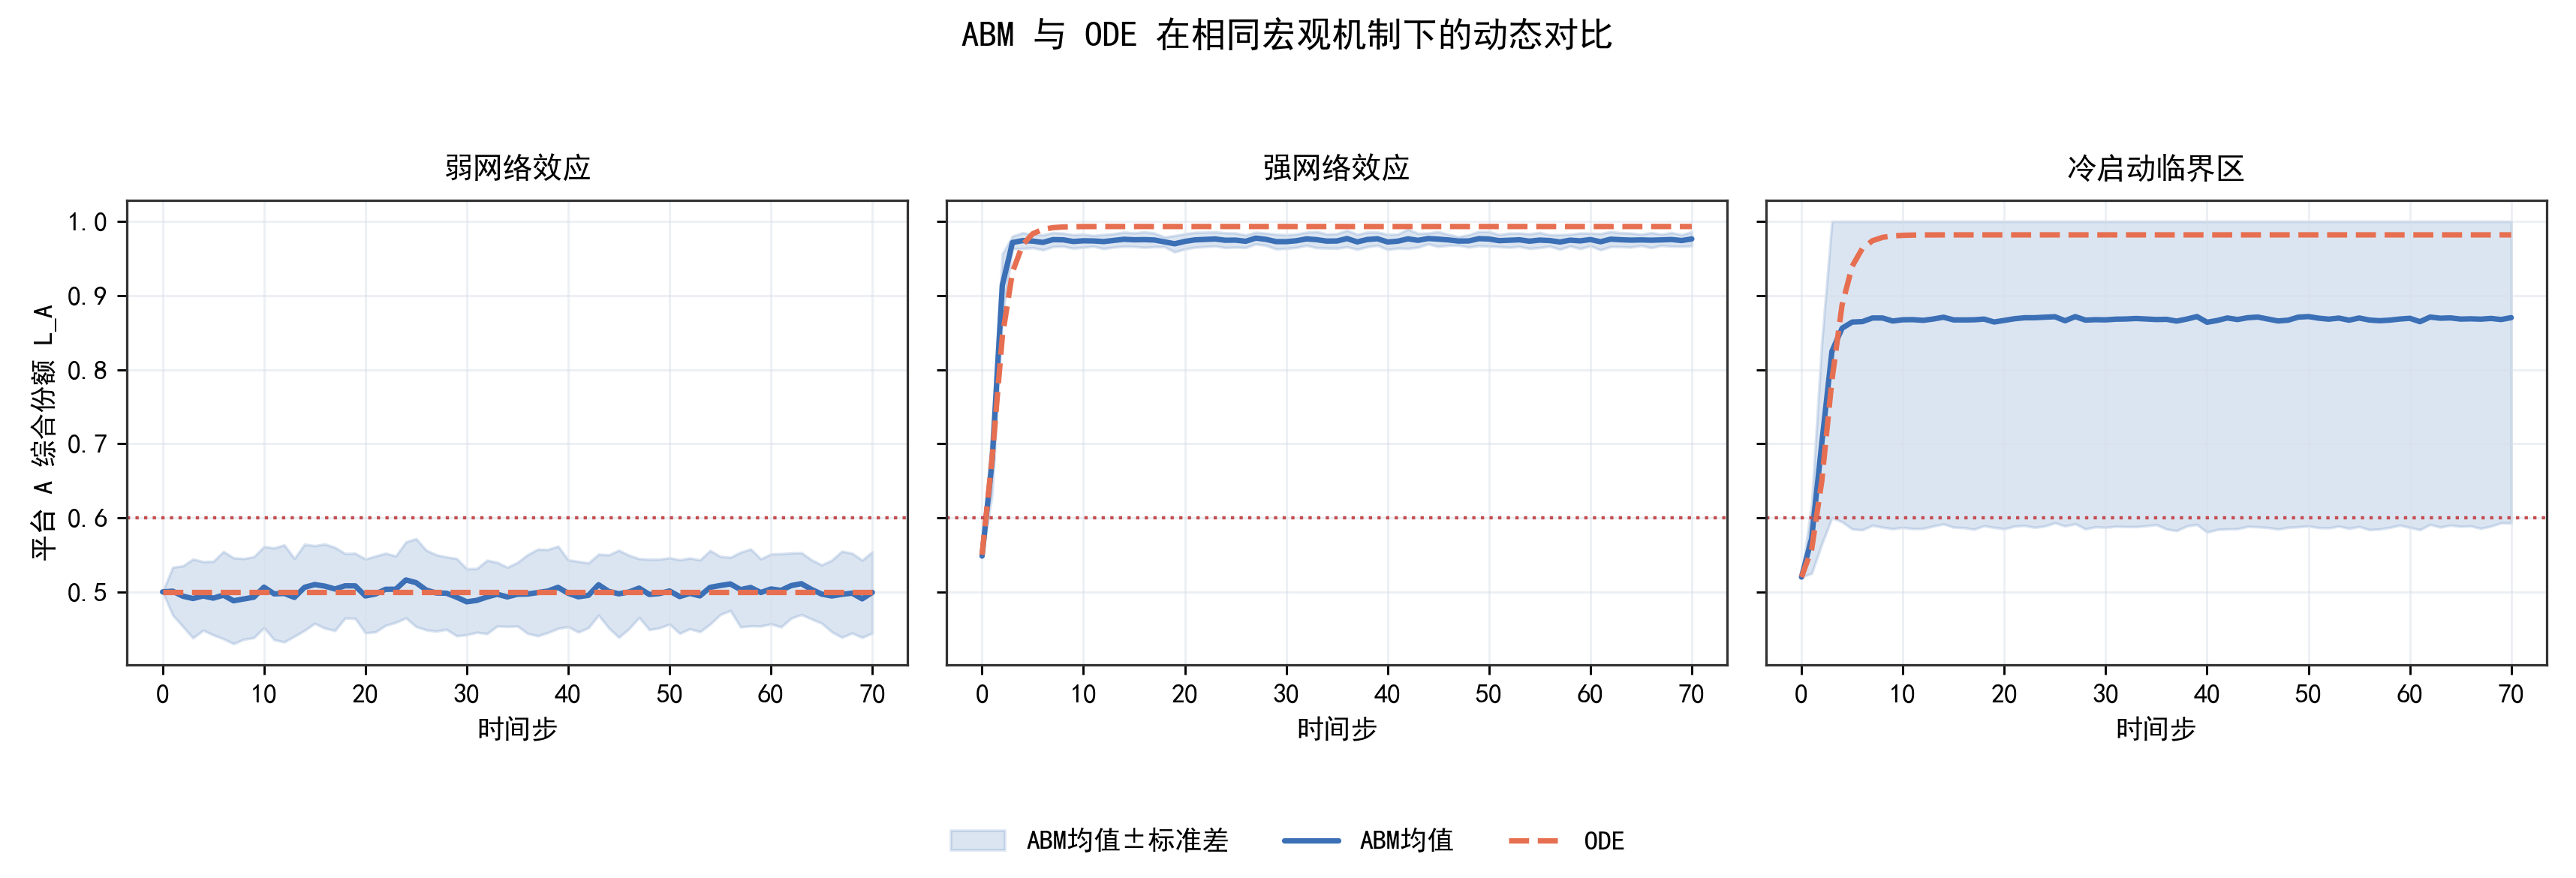
\includegraphics[width=\textwidth]{abm_ode_model_compare_paths.png}
    \caption{动态路径对比}
  \end{subfigure}
  \hfill
  \begin{subfigure}{0.34\textwidth}
    \centering
    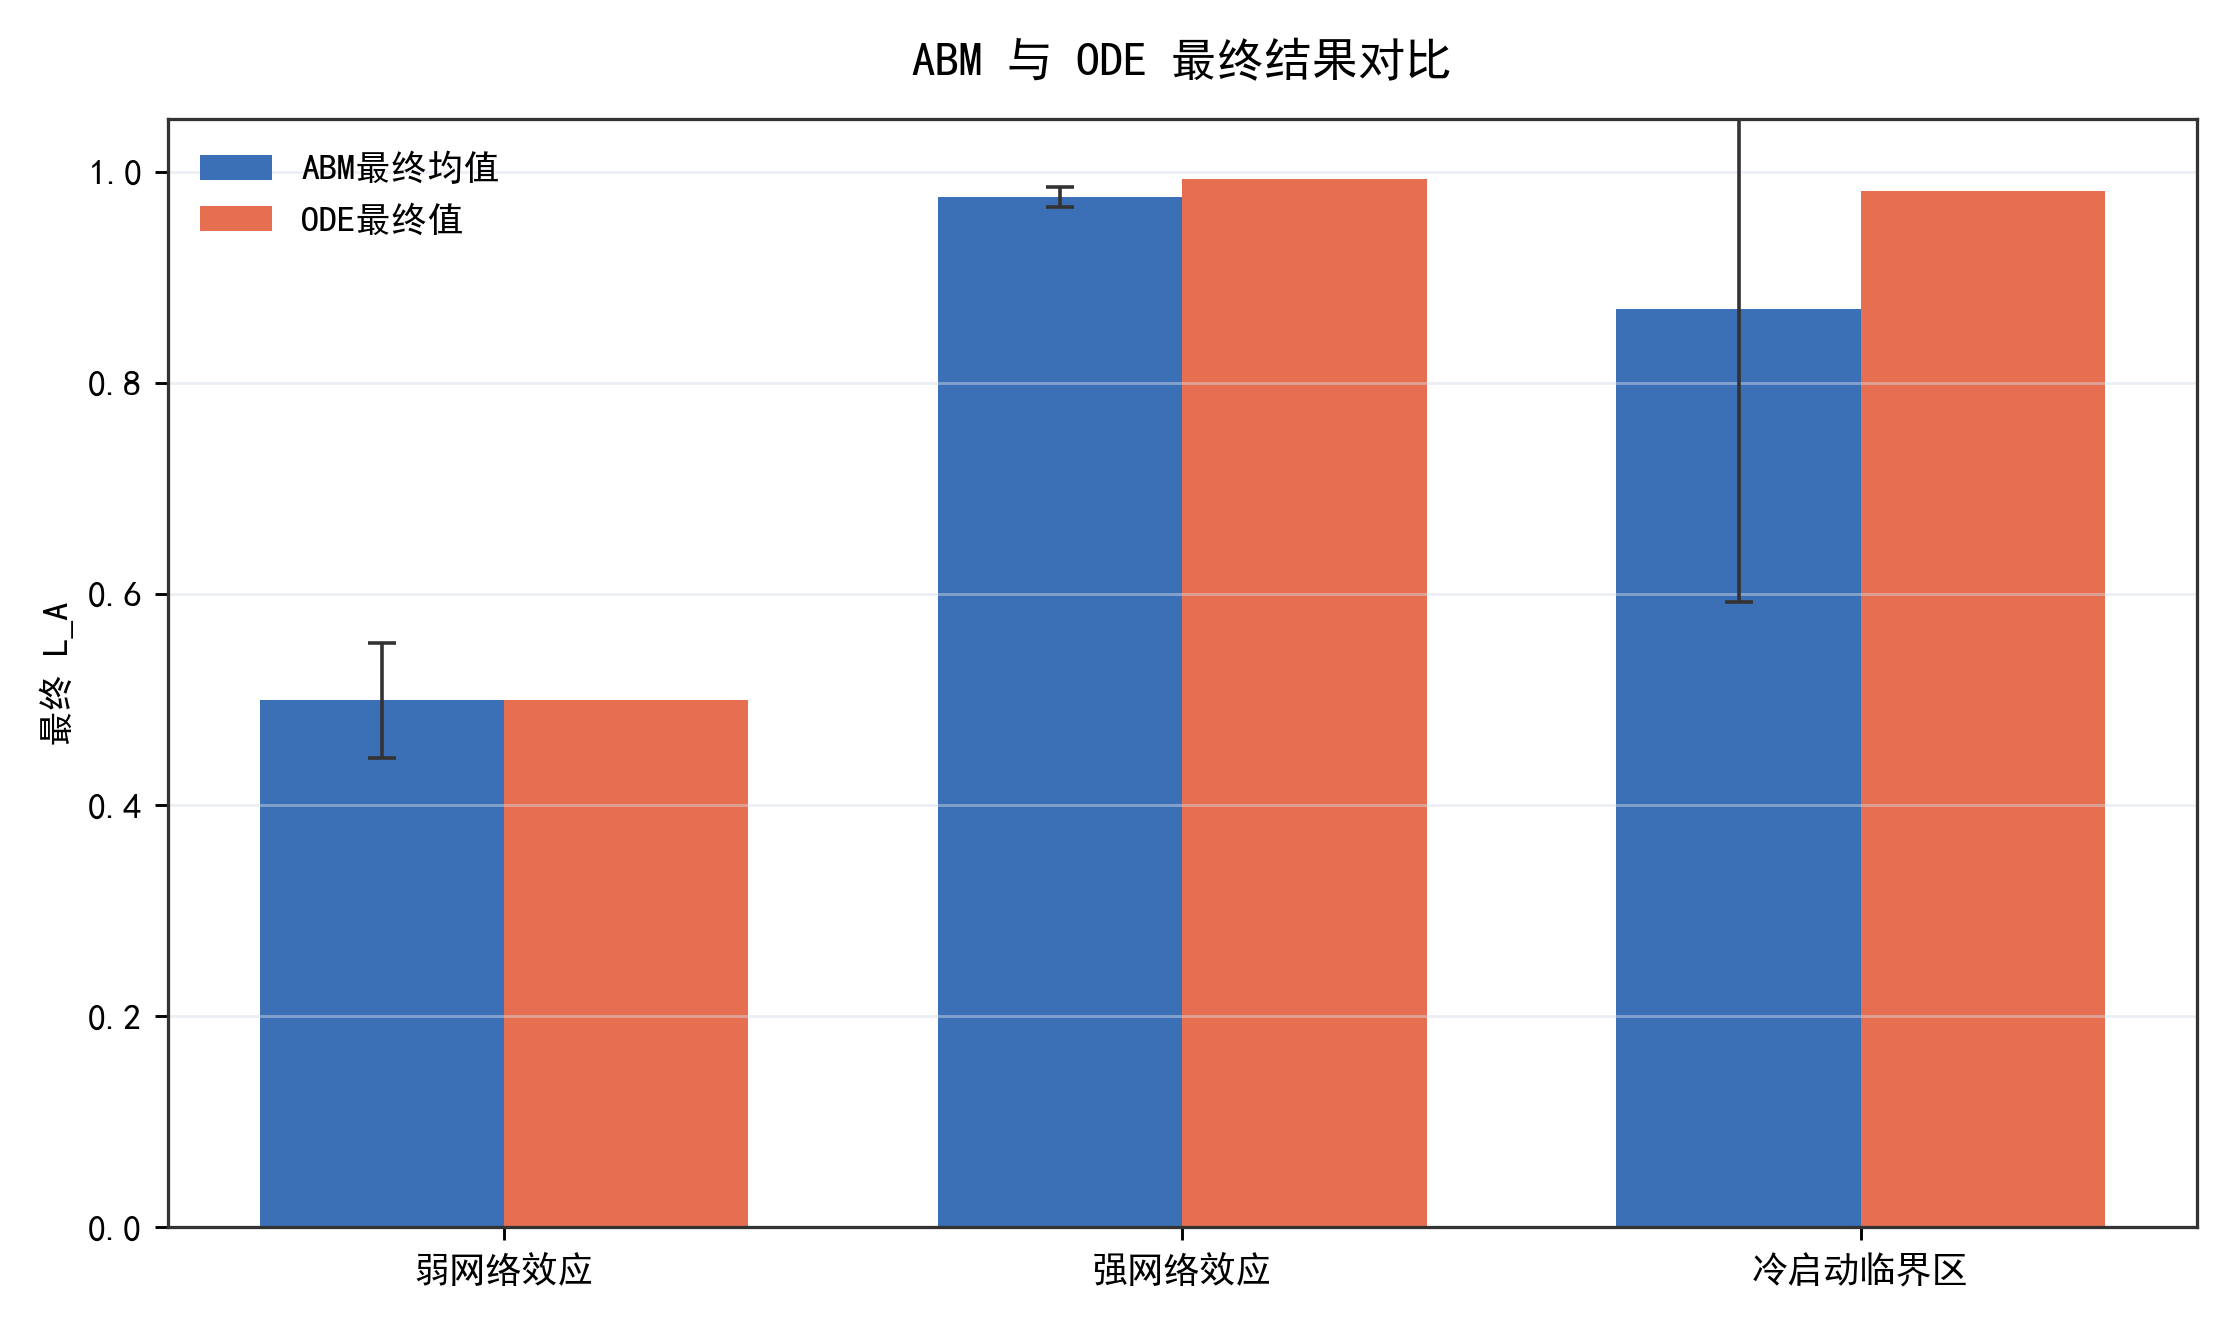
\includegraphics[width=\textwidth]{abm_ode_model_compare_final.png}
    \caption{最终结果对比}
  \end{subfigure}
  \caption{ABM 与 ODE 的结果对比}
  \label{fig:abm-ode}
\end{figure}

\begin{table}[H]
\centering
\caption{ABM 与 ODE 的最终结果比较}
\label{tab:abm-ode}
\begin{tabular}{lrrrr}
\toprule
场景 & ABM $\bar L_A$ & ABM $sd(L_A)$ & ODE $L_A$ & ABM 成功概率 \\
\midrule
弱网络效应 & 0.499 & 0.055 & 0.500 & 0.000 \\
强网络效应 & 0.976 & 0.010 & 0.993 & 1.000 \\
冷启动临界区 & 0.870 & 0.277 & 0.982 & 0.900 \\
\bottomrule
\end{tabular}
\end{table}

结果显示，在弱网络效应场景下，ODE 和 ABM 都收敛到接近 0.5 的共存状态，说明当交叉网络效应较弱时，微观随机性不足以形成系统性锁定。在强网络效应场景下，二者都显示平台 A 由轻微初始优势走向高份额锁定，ABM 最终均值为 0.976，ODE 最终值为 0.993，趋势高度一致。

差异主要出现在冷启动临界区。ODE 的最终 $L_A$ 为 0.982，表现为确定性地走向平台 A 优势；ABM 的均值为 0.870，但标准差达到 0.277，成功概率为 0.900。这说明在临界区，平均场模型容易给出较平滑、较确定的跃迁判断，而 ABM 揭示了个体异质性和随机路径导致的结果分布：同样的宏观参数下，大部分路径会成功跨越临界区，但仍存在少数路径未能形成锁定。因此，ABM 的核心贡献不是推翻 ODE，而是在 ODE 识别出的临界区域内进一步估计成功概率、波动范围和机制来源。

\section{综合讨论}

四组实验共同说明，双边平台竞争的关键不只是网络效应强弱，而是多个微观机制在临界区的叠加。

首先，个体异质性具有双重作用。中等异质性会使部分高敏感主体率先响应初始优势，增强领先平台的正反馈；强异质性则会使偏好分散化，降低最终市场集中度。其次，补贴不应只看总量，策略投向更重要。双边精准补贴能够同时激活用户侧和商户侧，使平台更早跨过临界规模。再次，冷启动具有明显的双边互补性。用户和商户资源必须共同达到一定水平，单边资源过强并不能完全替代另一侧缺口。最后，商户多归属降低了供给侧排他性，有助于平台共存，但这一作用依赖足够低的多归属成本和适度的有效供给贡献。

\section{现实印证与策略建议}

\subsection{可与现实平台竞争相互印证的结论}

第一，平台竞争存在明显的临界规模。实验 B 和实验 C 均显示，平台份额并不是随投入线性增长的。当用户侧和商户侧资源都低于临界区间时，补贴和拉新很难改变最终格局；但当双边资源同时接近阈值时，平台份额可能快速跃迁。现实中的外卖、网约车、电商和本地生活平台也呈现类似特征：早期竞争的关键不是单纯获得某一侧规模，而是推动用户侧需求和商户侧供给同时达到能够自我强化的最低规模。

第二，双边精准补贴比单边粗放补贴更有效。实验 B 表明，在相同预算下，同时补贴摇摆用户和关键商户能够显著降低跨越临界规模所需预算。现实中，平台通常不会长期平均补贴所有主体，而是更倾向于识别高频用户、价格敏感用户、可能迁移用户，以及能够带动品类供给和区域流量的关键商户。这与实验中双边精准补贴优于统一补贴和随机补贴的结论一致。

第三，商户多归属能够削弱平台锁定，但其效果取决于多归属成本。实验 D 显示，低成本多归属有助于平台共存；当多归属成本上升时，商户更容易转向单一平台，市场也更容易走向锁定。现实中，商户同时入驻多个外卖、电商或内容交易平台，是降低经营风险和扩大客源的重要方式；但如果平台通过复杂运营规则、排他协议、流量绑定或高管理成本提高多归属成本，市场集中和平台锁定会被强化。

第四，用户和商户的异质性会改变市场集中程度。实验 A 表明，中等异质性可能放大领先平台优势，而强异质性则可能降低市场集中度。现实中，如果用户需求高度一致，市场更容易向单个平台集中；如果用户在价格、服务质量、配送速度、品牌偏好和品类需求上差异较大，差异化平台就更容易获得生存空间。

\subsection{对平台的建议}

平台应将竞争重点从单边规模扩张转向双边临界规模管理。对于新平台或弱势平台，早期策略不应只追求用户注册量或商户入驻量，而应识别能够形成正反馈的用户--商户组合。例如，先在有限城市、有限品类或有限场景中获取足够密度的活跃用户和关键供给，再逐步扩展到更大市场。

补贴策略应减少平均主义投放，更多采用面向关键主体的定向投放。用户侧可以重点补贴高频、价格敏感、迁移概率高的用户；商户侧可以优先扶持品类标杆、区域核心商户和流量敏感型商户。补贴的目标不只是提升短期交易额，而是帮助平台跨过双边网络效应的启动阈值。

平台还应谨慎使用排他和强绑定策略。短期看，排他机制可能强化平台锁定；但长期看，过高的多归属成本会降低商户活跃度，削弱供给多样性，并可能带来监管和声誉风险。相比提高退出成本，更稳妥的做法是通过履约效率、数据工具、流量分发、公平规则和服务能力提高商户留存。

\subsection{对商家的建议}

商家在平台竞争尚未稳定时，应尽量保持适度多归属经营。多平台经营能够扩大客源、比较不同平台的转化率和费用结构，并降低被单一平台规则或流量机制锁定的风险。尤其在外卖、电商和本地生活场景中，多归属可以提高商家对平台抽成、广告费用和活动规则的议价能力。

但是，多归属也需要计算真实成本。商家应综合比较不同平台带来的订单增量、佣金、广告投入、履约成本、客服成本和运营复杂度。如果某个平台的边际收益不足以覆盖多平台经营成本，则应降低投入或调整资源分配。

对于具有稀缺供给能力的关键商户，应充分利用平台竞争窗口争取更好的合作条件。实验结果说明，关键商户会影响平台冷启动和补贴效率，因此优质商户可以在平台扩张期争取更合理的费率、流量扶持、服务工具和长期合作条款。

\subsection{对用户的建议}

用户应认识到平台补贴通常具有阶段性。竞争激烈或平台接近临界规模时，用户可以获得较高补贴和较低价格；但当市场逐渐锁定后，补贴可能下降，价格、会员规则和服务条款也可能变化。因此，用户保留多平台使用习惯，有助于降低被单一平台锁定的成本。

用户在选择平台时不应只关注短期补贴，也应关注商户供给质量、履约稳定性、售后机制和规则透明度。实验 C 表明，平台能否长期稳定发展取决于用户侧与商户侧资源是否匹配。如果平台补贴较高但供给不足、履约不稳定或服务质量较差，长期使用价值可能有限。

此外，用户选择会影响平台生态。持续选择服务质量较好、规则透明、商户供给稳定的平台，有助于推动平台从单纯补贴竞争转向效率、服务和生态质量竞争。

\section{结论}

本文基于 Mesa 构建了双边平台竞争 ABM，并通过多组重复实验得到以下结论：

\begin{enumerate}
  \item 个体异质性会改变市场锁定概率和集中度，其作用具有非线性。
  \item 补贴存在临界预算；在当前参数下，双边精准补贴的临界预算约为 160，统一补贴和随机补贴约为 200。
  \item 冷启动成功区域主要由用户侧和商户侧初始资源共同决定，商户供给侧对启动边界具有明显支撑作用。
  \item 种子质量和黏性可显著降低冷启动所需的初始规模。
  \item 低成本多归属有助于平台共存；当多归属成本升至约 0.4--0.5 后，共存概率快速接近 0。
  \item 机制消融表明，双边网络效应和商户多归属是弱势平台跨越临界区的主要支撑；惯性更多影响锁定强度。
  \item ABM 与 ODE 在弱网络和强网络场景下趋势一致，但 ABM 在冷启动临界区显示更大的路径波动和结果分布。
\end{enumerate}

这些结果说明，ABM 能够在微观主体差异、路径依赖和策略干预之间建立可解释联系，为双边平台竞争策略评估提供比单一均值模型更丰富的实验依据。

\section*{代码与数据文件}

实验代码入口为：
\begin{verbatim}
cd .\zl\AgentBasedModel_Mesa
python .\run_abm_experiments.py
\end{verbatim}

核心模型文件包括 \texttt{abm\_experiment\_model.py} 和 \texttt{run\_abm\_experiments.py}。本文图像来自 \texttt{results/figures}，结果表来自 \texttt{results/tables}。

\end{document}

